%%
%% This is file `sample-sigconf.tex',
%% generated with the docstrip utility.
%%
%% The original source files were:
%%
%% samples.dtx  (with options: `sigconf')
%% 
%% IMPORTANT NOTICE:
%% 
%% For the copyright see the source file.
%% 
%% Any modified versions of this file must be renamed
%% with new filenames distinct from sample-sigconf.tex.
%% 
%% For distribution of the original source see the terms
%% for copying and modification in the file samples.dtx.
%% 
%% This generated file may be distributed as long as the
%% original source files, as listed above, are part of the
%% same distribution. (The sources need not necessarily be
%% in the same archive or directory.)
%%
%% Commands for TeXCount
%TC:macro \cite [option:text,text]
%TC:macro \citep [option:text,text]
%TC:macro \citet [option:text,text]
%TC:envir table 0 1
%TC:envir table* 0 1
%TC:envir tabular [ignore] word
%TC:envir displaymath 0 word
%TC:envir math 0 word
%TC:envir comment 0 0
%%
%%
%% The first command in your LaTeX source must be the \documentclass command.


% Fixing: Too many math alphabets used in version normal.
\newcommand\hmmax{0}
\newcommand\bmmax{0}
\documentclass[utf8,acmsmall,review,screen,dvipsnames]{acmart}

\usepackage[colorinlistoftodos]{todonotes}
\usepackage[inference]{semantic}
\usepackage{fontawesome5}
\usepackage{listofitems}
\usepackage{glossaries}
\usepackage{cleveref}
\usepackage{stmaryrd}
\usepackage{marvosym}
\usepackage{listings}
\usepackage{xspace}
\usepackage{xfrac}
\usepackage{tikz}
\usepackage{bm}

% https://tex.stackexchange.com/questions/648845/sans-serif-uppercase-greek-no-longer-showing-in-acmart
\DeclareMathAlphabet{\mathsf}{OT1}{LibertinusSans-LF}{m}{n}
\SetMathAlphabet{\mathsf}{bold}{OT1}{LibertinusSans-LF}{bx}{n}

\DeclareMathAlphabet{\mathtt}{OT1}{lmtt}{m}{n}
\SetMathAlphabet{\mathtt}{bold}{OT1}{lmtt}{bx}{n}


\usetikzlibrary{calc,decorations.pathmorphing,shapes,positioning}
\newcounter{sarrow}
\newcommand\xrsquigarrow[1]{%
\stepcounter{sarrow}%
\mathrel{\begin{tikzpicture}[baseline= {( $ (current bounding box.south) + (0,-0.5ex) $ )}]
\node[inner sep=.5ex] (\thesarrow) {$\scriptstyle #1$};
\path[draw,<-,decorate,
  decoration={zigzag,amplitude=0.7pt,segment length=1.2mm,pre=lineto,pre length=4pt}]
    (\thesarrow.south east) -- (\thesarrow.south west);
\end{tikzpicture}}%
}
\makeatletter
\newcommand{\xRightarrow}[2][]{\ext@arrow 0359\Rightarrowfill@{#1}{#2}}
\makeatother

\newcommand{\thmref}[1]{\cref{#1}~(\nameref{#1})}
\newcommand{\Thmref}[1]{\Cref{#1}~(\nameref{#1})}

%%%%
% TODO macros
\newcommand{\MK}[1]{\todo[color=orange!30]{TODO: #1}}
\newcommand{\MKin}[1]{\todo[color=orange!30,inline]{TODO: #1}}
\newcommand{\MP}[1]{\todo[color=blue!30]{TODO: #1}}
\newcommand{\MPin}[1]{\todo[color=blue!30,inline]{TODO: #1}}
\newcommand{\hltt}[1]{\begin{center}\fbox{\color{green}\large{#1}}\end{center}}

% Approx
\newcommand{\pages}[1]{}%\xspace\todo{\textbf{($\sim$#1 pages)}\xspace}}

%%%%
% Colors
\newcommand{\neutcol}[0]{black}
\newcommand{\stlccol}[0]{RoyalBlue}
\newcommand{\irccol}[0]{Apricot}
\newcommand{\ulccol}[0]{RedOrange}
\newcommand{\objcol}[0]{Emerald} %CarnationPink}
\newcommand{\commoncol}[0]{black}

\newcommand{\col}[2]{\ensuremath{{\color{#1}{#2}}}}

\newcommand{\com}[1]{\ensuremath\mathit{\col{\neutcol}{#1}}}
\newcommand{\src}[1]{\ensuremath\mathsf{\col{\stlccol}{#1}}}
\newcommand{\irl}[1]{\ensuremath\mathit{\col{\irccol}{#1}}}
\newcommand{\trg}[1]{\ensuremath\mathbf{\col{\ulccol}{#1}}}
\newcommand{\obj}[1]{\ensuremath\mathtt{\col{\objcol}{#1}}}

%%%%
% Text Decorations
\newcommand\BrText[2]{%
  \par\smallskip
   \noindent\makebox[\textwidth][r]{$\text{\scriptsize #1}\left\{
    \begin{minipage}{\textwidth}
    #2
    \end{minipage}
  \right.\nulldelimiterspace=0pt$}\par\smallskip
}
\newcommand{\mi}[1]{\ensuremath{\mathit{#1}}}
\newcommand{\mr}[1]{\ensuremath{\mathrm{#1}}}
\newcommand{\mt}[1]{\ensuremath{\texttt{#1}}}
\newcommand{\mtt}[1]{\ensuremath{\mathtt{#1}}}
\newcommand{\mf}[1]{\ensuremath{\mathbf{#1}}}
\newcommand{\mk}[1]{\ensuremath{\mathfrak{#1}}}
\newcommand{\mc}[1]{\ensuremath{\mathcal{#1}}}
\newcommand{\ms}[1]{\ensuremath{\mathsf{#1}}}
\newcommand{\mb}[1]{\ensuremath{\mathbb{#1}}}
\newcommand{\msc}[1]{\ensuremath{\mathscr{#1}}}

\newcommand{\bul}[1]{{\setulcolor{RoyalBlue}\ul{#1}}}
\newcommand{\rul}[1]{{\setulcolor{RedOrange}\ul{#1}}}
\newcommand{\iul}[1]{{\setulcolor{Apricot}\ul{#1}}}
\newcommand{\oul}[1]{{\setulcolor{Emerald}\ul{#1}}}
\newcommand{\pul}[1]{{\setulcolor{CarnationPink}\ul{#1}}}

\newcommand{\lock}{\ensuremath\text{\scriptsize\faIcon{lock}}}
\newcommand{\unlock}{\ensuremath\text{\scriptsize\faIcon{lock-open}}}

\newcommand{\tup}[2]{\ensuremath (#1 %
  \readlist\myterms{#2}%
  \foreachitem\x\in\myterms{;\x}%
  )%
}

\newcommand{\isdef}[0]{\ensuremath{\mathrel{\overset{\makebox[0pt]{\mbox{\normalfont\tiny\sffamily def}}}{=}}}}

%%%%
% List of contributions
\newcounter{contrib}
\newcommand{\contribnum}[0]{\stepcounter{contrib}{\arabic{contrib}}.~}
\newcommand{\contribution}[1]{\smallskip\noindent\textbf{{#1.}\xspace}}

%%%%
% A symbol for Coq-verified theorems.
\newcommand{\BareCoqSymbol}{
\includegraphics[height=0.9em]{coq.pdf}}
\newcommand{\CoqSymbol}{\raisebox{-.2ex}{\BareCoqSymbol\,}}
\newcommand{\Coqed}{\hfill\CoqSymbol}

\newcommand{\BareInvCoqSymbol}{
\includegraphics[height=0.9em]{inv_coq.png}}
\newcommand{\InvCoqSymbol}{\raisebox{-.2ex}{\BareInvCoqSymbol\,}}

%%%%
% Typerules
\newcommand{\textgraybox}[1]{\boxed{#1}}
\newdimen\zzfontsz
\newcommand{\fontsz}[2]{\zzfontsz=#1%
{\fontsize{\zzfontsz}{1.2\zzfontsz}\selectfont{#2}}}
\newcommand{\mathsz}[2]{\text{\fontsz{#1}{$#2$}}}
\newcommand{\instsymColon}{%
     \raisebox{-0.09ex}{\text{\normalfont{:}}}}
\newcommand{\judgboxfontsize}[1]{%
        \mathsz{11pt}{#1}%
}
\newcommand{\judgbox}[2]{%
      {\raggedright \textgraybox{\ensuremath{\judgboxfontsize{#1}}}\!%
        \fontsz{9pt}{\begin{tabular}[c]{l} #2 \end{tabular}} %
}}
\newcounter{typerule}
\crefname{typerule}{rule}{rules}

\newcommand{\typeruleInt}[5]{%
	\def\thetyperule{#1}%
	\refstepcounter{typerule}%
	\label{tr:#4}%
	%
  \ensuremath{\begin{array}{c}#5 \inference{#2}{#3}\end{array}}
}
\newcommand{\typerule}[4]{%
  \typeruleInt{#1}{#2}{#3}{#4}{\textsf{\scriptsize ({#1})} \\      }
}
\newcommand{\typerulenolabel}[3]{%
	\def\thetyperule{#1}%
	\refstepcounter{typerule}%
  \ensuremath{\begin{array}{c} \inference{#2}{#3}\end{array}}
}
\newcommand{\typerulederiv}[3]{%
  \ensuremath{\begin{array}{c} \inference{#2}{#3} #1\end{array}}
}

%%%%
% Language-specific definitions
% names of properties
\newcommand{\tmssafe}{\ensuremath\operatorname{tms}}
\newcommand{\smssafe}{\ensuremath\operatorname{sms}}
\newcommand{\mssafe}{\ensuremath\operatorname{ms}}
\newcommand{\scctsafe}{\ensuremath\operatorname{scct}}
\newcommand{\msscctsafe}{\ensuremath\operatorname{msscct}}

% Languages
\newcommand{\Ltms}{\ensuremath\src{L_{\tmssafe}}}
\newcommand{\Ltrg}{\ensuremath\trg{L}}
\newcommand{\Lms}{\ensuremath\irl{L_{\mssafe}}}
\newcommand{\Lscct}{\ensuremath\obj{L_{\scctsafe}}}

% Traces
\newcommand{\event}[1][]{a#1}
\newcommand{\absevent}[1][]{\ensuremath\bm{\event[#1]}}
\newcommand{\emptyevent}{\ensuremath\varepsilon}
\newcommand{\trace}[1][]{\ensuremath\overline{a#1}}
\newcommand{\class}[1][]{\ensuremath\mb{C}}
\newcommand{\lift}[1]{\ensuremath\lfloor\xspace{#1}\xspace\rfloor}
\newcommand{\hole}[1]{\ensuremath{\left[#1\right]}}
\newcommand{\ev}[1]{\text{#1}}
\newcommand{\absev}[1]{\ensuremath\bm{#1}}
\newcommand{\abstrace}[1][]{\ensuremath\bm{\trace[]}#1}
\newcommand{\absterm}{\ensuremath\lightning{\kern-5.5pt}\lightning}

% Trace Relations
\newcommand{\traceagree}[4][^*]{\ensuremath{#3}\cong_{#2}#1{#4}}
\newcommand{\tmstraceagree}[3][^*]{\traceagree[#1]{\tmssafe}{#2}{#3}}
\newcommand{\smstraceagree}[3][^*]{\traceagree[#1]{\smssafe}{#2}{#3}}
\newcommand{\mstraceagree}[3][^*]{\traceagree[#1]{\mssafe}{#2}{#3}}
\newcommand{\sccttraceagree}[3][^*]{\traceagree[#1]{\scctsafe}{#2}{#3}}

% Monitors
\newcommand{\monitor}[1][]{\ensuremath T#1}
\newcommand{\tmsmonitor}[1][]{\monitor[_{TMS}{#1}]}
\newcommand{\smsmonitor}[1][]{\monitor[_{SMS}{#1}]}
\newcommand{\scctmonitor}[1][]{\monitor[_{sCCT}{#1}]}
\newcommand{\msmonitor}[1][]{\monitor[_{MS}{#1}]}
\newcommand{\monitorcheck}[4][{\kern-3.5pt}^*]{%
  \vdash\xspace{#2}\xspace \xrsquigarrow{#4}{#1}\xspace{#3}\xspace%
}
\newcommand{\monsafe}[2]{\ensuremath\vdash_{mon}{#1}:{#2}}

\newcommand{\abssecuritytag}[1][]{\ensuremath\bm{\sigma}#1}

\newcommand{\montmssafe}[1]{\monsafe{#1}{\tmssafe}}
\newcommand{\monsmssafe}[1]{\monsafe{#1}{\smssafe}}
\newcommand{\monmssafe}[1]{\monsafe{#1}{\mssafe}}
\newcommand{\monscctsafe}[1]{\monsafe{#1}{\scctsafe}}
\newcommand{\monmsscctsafe}[1]{\monsafe{#1}{\msscctsafe}}

% Languages
\newcommand{\LTMS}{\src{L_{TMS}}}
\newcommand{\LT}{\trg{L}}
\newcommand{\LMS}{\irl{L_{MS}}}
\newcommand{\LCCT}{\obj{L_{sCCT}}}

\newcommand{\bnfdef}{\ensuremath{\mathrel{::=}}}

% Substitution
\newcommand{\subst}[2]{\ensuremath \hole{#1\text{ for }#2}}
\newcommand{\substvar}[1][]{\ensuremath \gamma#1}
\newcommand{\substlist}[1][]{\ensuremath \overline{\gamma#1}}

\newcommand{\partialeval}[2]{\ensuremath \operatorname{\mathtt{mix}}(#1, #2)}

% Predefined Sets
\newcommand{\nat}{\ensuremath\mb{N}}

% Types
\newcommand{\natt}{\ensuremath\mb{N}_t\xspace}
\newcommand{\ptrqual}[1][]{\ensuremath\xspace q#1\xspace}
\newcommand{\fullq}{1\xspace}
\newcommand{\halfq}{\sfrac{1}{2}\xspace}
\newcommand{\ptrn}[1][\ptrqual]{\ensuremath\xspace ref_{#1}\ \natt\xspace}
\newcommand{\wptr}{\ensuremath\ptrn[\halfq]\xspace}
\newcommand{\ptr}{\ensuremath\ptrn[\fullq]\xspace}
\newcommand{\type}[1][]{\ensuremath\tau#1\xspace}
\newcommand{\typenv}[1][]{\ensuremath\Gamma#1\xspace}

% Terms
\newcommand{\wrapkeyword}[2][]{\ensuremath{#1{#2}}}
\newcommand{\expr}[1][]{e#1\xspace}
\newcommand{\ectx}[1][]{K#1\xspace}
\newcommand{\finalexpr}[1][]{f#1\xspace}
\newcommand{\valueexpr}[1][]{v#1\xspace}
\newcommand{\lbinop}[3][]{\ensuremath {#2}{#1{\oplus}}{#3}\xspace}
\newcommand{\lget}[3][]{\ensuremath #2{#1{[}}{#3}{#1{]}}\xspace}
\newcommand{\lset}[4][]{\ensuremath #2{#1{[}}{#3}{#1{]\leftarrow}}#4\xspace}
\newcommand{\lnew}[3][]{\ensuremath \wrapkeyword[#1]{new}\ #2\ {#1{[}}#3{#1{]}}\xspace}
\newcommand{\llet}[4][]{\ensuremath \wrapkeyword[#1]{let}\ #2 {#1{=}} #3\ \wrapkeyword[#1]{in}\ #4\xspace}
\newcommand{\ldelete}[2][]{\ensuremath \wrapkeyword[#1]{delete}\ #2\xspace}
\newcommand{\lreturn}[2][]{\ensuremath \wrapkeyword[#1]{return}\ #2\xspace}
\newcommand{\lcall}[3][]{\ensuremath \wrapkeyword[#1]{call}\ #2\ #3\xspace}
\newcommand{\lifz}[4][]{\ensuremath \wrapkeyword[#1]{ifz}\ #2\ \wrapkeyword[#1]{then}\ #3\ \wrapkeyword[#1]{else}\ #4\xspace}
\newcommand{\labort}[1][]{\ensuremath \wrapkeyword[#1]{abort()}\xspace}
\newcommand{\lispoisoned}[2][]{\ensuremath #2\ \wrapkeyword[#1]{is\ }{#1{\poisoned}}\xspace}
\newcommand{\lpair}[3][]{\ensuremath {#1{\langle}} #2 {#1{;}} #3 {#1{\rangle}} \xspace}
\newcommand{\lproja}[2][]{\ensuremath {#2}{#1{.0}} \xspace}
\newcommand{\lprojb}[2][]{\ensuremath {#2}{#1{.1}} \xspace}
\newcommand{\lhast}[3][]{\ensuremath {#2}\ \wrapkeyword[#1]{has}\ #3 \xspace}
\newcommand{\lwrdoit}[2][]{\ensuremath \wrapkeyword[#1]{wrdoit}\ #2\xspace}
\newcommand{\lrddoit}[3][]{\ensuremath \wrapkeyword[#1]{rddoit}\ #2\ \wrapkeyword[#1]{in}\ #3\xspace}
\newcommand{\function}[1][]{F#1\xspace}
\newcommand{\lfunction}[4][]{\ensuremath\wrapkeyword[#1]{fn}\ {#2}\ {#3}\ {#1{:=}}\ #4\xspace}
\newcommand{\prog}[3][]{\ensuremath\wrapkeyword[#1]{\langle}\ #2; #3\wrapkeyword[#1]{\rangle}\xspace}

% Compiler
\newcommand{\rtp}[2]{\ensuremath\vdash{#1}:{#2}}
\newcommand{\ccbase}[1][]{\ensuremath\gamma{#1}}
\newcommand{\cc}[3][]{\ensuremath{\ccbase[#1]}^{#2}_{#3}\xspace}
\newcommand{\cca}{\ensuremath\cc{\Ltms}{\Ltrg}}
\newcommand{\ccb}{\ensuremath\cc{\Ltrg}{\Lms}}
\newcommand{\ccdce}{\ensuremath\cc[_{\gls{dce}}]{\Lms}{\Lms}}
\newcommand{\cccf}{\ensuremath\cc[_{\gls{cf}}]{\Lms}{\Lms}}
\newcommand{\ccscct}{\ensuremath\cc{\Lms}{\Lscct}}
\newcommand{\ccmsscct}{\ensuremath\cc{\Ltms}{\Lscct}}

% Backtranslation
\newcommand{\backbase}[1][]{\ensuremath\wp#1}
\newcommand{\backt}[3][]{\ensuremath{}^{#2}_{#3}\backbase[#1]}

% Satisfaction
\newcommand{\contextvar}[1][]{C#1}
\newcommand{\progvar}[1][]{p#1}
\newcommand{\wholeprogvar}[1][]{w#1}
\renewcommand{\class}[1][]{\mathbb{C}#1}
\newcommand{\link}[2]{\ensuremath\operatorname{link}\left({#1};{#2}\right)}
\newcommand{\behav}[1]{\ensuremath\operatorname{behav}\left({#1}\right)}
\newcommand{\sat}[2]{\ensuremath\vdash{#1}:{#2}}
\newcommand{\rsat}[2]{\ensuremath\vdash_R{#1}:{#2}}

% State
\newcommand{\securitytag}[1][]{\ensuremath\sigma#1}
\newcommand{\sandboxtag}[1][]{t#1}
\newcommand{\ctx}{\text{ctx}}
\newcommand{\comp}{\text{comp}}
\newcommand{\loc}[1][]{\ensuremath l#1}
\newcommand{\poison}{\ensuremath\rho}
\newcommand{\poisoned}{\ensuremath\text{\Biohazard}}
\newcommand{\poisonless}{\ensuremath\square}
\newcommand{\store}[1][]{\ensuremath\Delta#1}
\newcommand{\storeel}[5]{\ensuremath #1\mapsto\tup{#2}{#3,#4,#5}}
\newcommand{\comm}[1][]{\ensuremath c#1}
\newcommand{\ctxtocomp}{\ensuremath\xspace ? \xspace}
\newcommand{\comptoctx}{\ensuremath\xspace ! \xspace}
\newcommand{\nocomm}{\ensuremath\xspace \varnothing \xspace}
\newcommand{\heap}[1][]{\ensuremath H#1}
\newcommand{\ectxstack}[1][]{\ensuremath\overline{\ectx#1}}
\newcommand{\library}[1][]{\ensuremath\Xi#1}
\newcommand{\commlib}[1][]{\ensuremath\xi#1}
\newcommand{\cfstate}[1][]{\ensuremath\Psi#1}
\newcommand{\memstate}[1][]{\ensuremath\Phi#1}
\newcommand{\statevar}[1][]{\ensuremath\Omega#1}
\newcommand{\rtt}[2]{\ensuremath #1 \triangleright #2}
\newcommand{\growh}[2]{\ensuremath #1 \ll #2}
\newcommand{\seth}[3]{\ensuremath #1(#2 \mapsto #3)}

% Various Judgements
\newcommand{\fresh}[2]{\ensuremath{#1}\vdash{#2}\xspace\operatorname{fresh}\xspace}
\newcommand{\tcheck}[3]{\ensuremath{#1}\vdash{#2}:{#3}\xspace}
\newcommand{\notowned}[1]{\ensuremath\vdash{#1}\xspace\operatorname{not-owned}\xspace}
\newcommand{\typenvsplit}[2]{\ensuremath {#1}\odot{#2}\xspace}
\newcommand{\hastype}[2]{\ensuremath{#1}:{#2}\xspace}
\newcommand{\inttype}[1]{\ensuremath\vdash{#1}\operatorname{int-\type}\xspace}

\newcommand{\thelocmap}{\ensuremath\delta\xspace}
\newcommand{\locmapsto}[2]{\ensuremath\thelocmap({#1})={#2}\xspace}

% Filters
\newcommand{\filter}[4][]{\ensuremath \operatorname{Proj}^{#1}_{#2}\left({#3}, {#4}\right)\xspace}
\newcommand{\msfilterLtms}[2][{\thelocmap}]{\ensuremath\filter[{\Ltms}]{}{#1}{#2}}
\newcommand{\msfilterLms}[2][{\thelocmap}]{\ensuremath\filter[{\Lms}]{}{#1}{#2}}
\newcommand{\msfilterL}[2][{\thelocmap}]{\ensuremath\filter[{\Ltrg}]{}{#1}{#2}}
\newcommand{\scctfilterLms}[2][{\thelocmap}]{\ensuremath\filter[{\Lms}]{}{#1}{#2}}
\newcommand{\scctfilterLscct}[2][{\thelocmap}]{\ensuremath\filter[{\Lscct}]{}{#1}{#2}}

% Steps
\newcommand{\isval}[1]{\ensuremath\vdash{#1}\xspace\operatorname{is-val}\xspace}
\newcommand{\runtimetermvar}[1][]{r#1}
\newcommand{\stepto}[4][{\kern-4.5pt}^*]{\ensuremath{#2}\xrightarrow{#4}{}\xspace{#1}\xspace{#3}\xspace}
\newcommand{\stepton}[4][n]{\ensuremath{#2}\xrightarrow{#4}{}{\kern-3.5pt}^{#1}\xspace{#3}\xspace}

\newcommand{\pstepto}[3]{\ensuremath{#1}\xrightarrow{#3}_p{}\xspace{#2}\xspace}
\newcommand{\estepto}[4][{\kern-4.5pt}^*]{\ensuremath{#2}\xrightarrow{#4}#1_{\operatorname{ectx}}\xspace{#3}\xspace}
\newcommand{\estepton}[4][n]{\ensuremath{#2}\xrightarrow{#4}_{\operatorname{ectx}}{}{\kern-14.5pt}^{#1\ \ \ \;}\xspace{#3}\xspace}
\newcommand{\progstepto}[3]{\ensuremath{#1}\xRightarrow{#3}{#2}}


\loadglsentries{acronyms}
\makeglossaries

%% NOTE that a single column version may be required for 
%% submission and peer review. This can be done by changing
%% the \doucmentclass[...]{acmart} in this template to 
%% \documentclass[manuscript,screen]{acmart}
%% 
%% To ensure 100% compatibility, please check the white list of
%% approved LaTeX packages to be used with the Master Article Template at
%% https://www.acm.org/publications/taps/whitelist-of-latex-packages 
%% before creating your document. The white list page provides 
%% information on how to submit additional LaTeX packages for 
%% review and adoption.
%% Fonts used in the template cannot be substituted; margin 
%% adjustments are not allowed.
%%
%%
%% \BibTeX command to typeset BibTeX logo in the docs
\AtBeginDocument{%
  \providecommand\BibTeX{{%
    \normalfont B\kern-0.5em{\scshape i\kern-0.25em b}\kern-0.8em\TeX}}}

%% Rights management information.  This information is sent to you
%% when you complete the rights form.  These commands have SAMPLE
%% values in them; it is your responsibility as an author to replace
%% the commands and values with those provided to you when you
%% complete the rights form.
\setcopyright{acmcopyright}
\copyrightyear{2024}
\acmYear{2024}
\acmDOI{XXXXXXX.XXXXXXX}

%% These commands are for a PROCEEDINGS abstract or paper.
\acmConference[POPL '24]{Make sure to enter the correct
  conference title from your rights confirmation emai}{June 03--05,
  2018}{Woodstock, NY}
%
%  Uncomment \acmBooktitle if th title of the proceedings is different
%  from ``Proceedings of ...''!
%
%\acmBooktitle{Woodstock '18: ACM Symposium on Neural Gaze Detection,
%  June 03--05, 2018, Woodstock, NY} 
\acmPrice{15.00}
\acmISBN{978-1-4503-XXXX-X/18/06}


%%
%% Submission ID.
%% Use this when submitting an article to a sponsored event. You'll
%% receive a unique submission ID from the organizers
%% of the event, and this ID should be used as the parameter to this command.
%%\acmSubmissionID{123-A56-BU3}

%%
%% For managing citations, it is recommended to use bibliography
%% files in BibTeX format.
%%
%% You can then either use BibTeX with the ACM-Reference-Format style,
%% or BibLaTeX with the acmnumeric or acmauthoryear sytles, that include
%% support for advanced citation of software artefact from the
%% biblatex-software package, also separately available on CTAN.
%%
%% Look at the sample-*-biblatex.tex files for templates showcasing
%% the biblatex styles.
%%

%%
%% The majority of ACM publications use numbered citations and
%% references.  The command \citestyle{authoryear} switches to the
%% "author year" style.
%%
%% If you are preparing content for an event
%% sponsored by ACM SIGGRAPH, you must use the "author year" style of
%% citations and references.
%% Uncommenting
%% the next command will enable that style.
\citestyle{acmauthoryear}

%%
%% end of the preamble, start of the body of the document source.
\begin{document}

%%
%% The "title" command has an optional parameter,
%% allowing the author to define a "short title" to be used in page headers.
\title{Secure Composition of Robust and Optimising Compilers}

%%
%% The "author" command and its associated commands are used to define
%% the authors and their affiliations.
%% Of note is the shared affiliation of the first two authors, and the
%% "authornote" and "authornotemark" commands
%% used to denote shared contribution to the research.
\author{Matthis Kruse}
% \authornote{Both authors contributed equally to this research.}
\email{matthis.kruse@cispa.de}
\orcid{0000-0003-4062-9666}
\affiliation{%
  \institution{CISPA Helmholtz Center for Information Security}
  \streetaddress{Stuhlsatzenhaus 5}
  \city{Saarbr{\"u}cken}
  \state{Saarland}
  \country{Germany}
  \postcode{66123}
}

\author{Marco Patrignani}
\orcid{0000-0003-3411-9678}
\email{marco.patrignani@unitn.it}
\affiliation{%
  \institution{University of Trento}
  \streetaddress{Via Sommarive, 9}
  \city{Povo}
  \country{Italy}
  \postcode{38123}
}

%%
%% By default, the full list of authors will be used in the page
%% headers. Often, this list is too long, and will overlap
%% other information printed in the page headers. This command allows
%% the author to define a more concise list
%% of authors' names for this purpose.
\renewcommand{\shortauthors}{Kruse and Patrignani}

%%
%% The abstract is a short summary of the work to be presented in the
%% article.
\begin{abstract}
  \hltt{abstract}

\begin{center}\small\it
	{This paper uses syntax highlighting accessible to both colourblind and black \& white readers~\citep{patrignani2020use}.
	Specifically, it makes use of a $\src{blue}$, $\src{sans\text{-}serif}$ font for a $\src{source}$,
	a $\trg{red}$, $\trg{bold}$ font for an $\trg{intermediate}$,
	and a $\obj{green}$, $\obj{teletype}$ font for a $\obj{target}$ language.
	}
\end{center}
\end{abstract}

%%
%% The code below is generated by the tool at http://dl.acm.org/ccs.cfm.
%% Please copy and paste the code instead of the example below.
%%
\begin{CCSXML}
<ccs2012>
  <concept>
  <concept_id>10002978.10002986.10002989</concept_id>
  <concept_desc>Security and privacy~Formal security models</concept_desc>
  <concept_significance>500</concept_significance>
  </concept>
</ccs2012>
\end{CCSXML}
\ccsdesc[500]{Security and privacy~Formal security models}

%%
%% Keywords. The author(s) should pick words that accurately describe
%% the work being presented. Separate the keywords with commas.
\keywords{Memory-safety, Secure Compilation, Privacy}

%%
%% This command processes the author and affiliation and title
%% information and builds the first part of the formatted document.
\maketitle

\section{Introduction}

\hltt{Context}
\hltt{Problem}

\BrText{Solution}{
% keyword: pass
\MPin{
	commands missing
}
This paper introduces a framework for reasoning about the composition of secure and optimising compiler passes and it showcases the power of this framework by instantiating it on a multi-pass compilation chain.
To this end, this paper first discusses how to compose security properties, such as temporal and spatial memory safety into general memory safety, and cryptographic constant time.
Then, this paper defines several secure compiler passes, where each is either preserving a different security property (e.g., temporal or spatial memory safety) or performing a security-preserving optimisation, (e.g., applying constant-folding or dead-code elimination).
% keyword- end to end, composition
Finally, this paper shows how to compose these secure compiler passes into a multi-pass compilation chain which can be proven to provide end-to-end preservation of general memory safety and cryptographic constant time.
\MKin{
  ,,can be proven'' -> is proven (?)
}
Crucially, this end-to-end security preservation is obtained by having each compilation pass (i) preserve a sub-part of the overall security property individually and then (ii) compose each preserved security property as dictated by the framework of this paper.
The results showcase how the framework allows the kind of formal security reasoning that compiler writers already want (and do), obtaining precise, compositional security reasoning while providing minimal (and modular) proof effort.
\MPin{
	last line: not the best.
}
}

% \BrText{Validation}{
In summary, this paper makes the following contributions:

\begin{itemize}
  \item %
        %\Cref{sec:compprop} presents a formal framework to reason about compositions of security properties and demonstrate its usage with concrete examples:
        First, this paper studies the formalisation and the composition of security properties (\Cref{sec:compprop}) by focussing on those safety properties that are of interest for real-world compiler writers (as identified by the plethora of work enforcing such properties individually~\MP{cits}).
        % 
        Starting from ways to formalise and enforce those properties individually, this paper shows how to compose both their formalisation and their composition.
        % 
        This paper then showcases the benefits of this composition by composing \gls{tms} and \gls{sms} into \gls{ms}, and ultimately adding \gls{cct} to the composition, yielding the the conjunction of \gls{ms} and \gls{cct}.
        % 
        The resulting security property is the golden standard of safety properties that secure cryptographic code should have~\MP{cits}.
        \MPin{
        	conclude that did this prop in a single pass, we show how to do it compositionally
        }
        %For each of these properties, we also give a monitor which runs on another trace model that excludes unneccessary information and show that their composition is behaviorally similar to the composition of the trace-based security properties.
        %This two-level approach enhances modularity: When working with the security properties, one only needs to reason about the corresponding monitor.
        %%% let's omit above sentences completely. why ramble about monitors in the introduction? this ain't about model checking

  \item %
        %\Cref{sec:compcomp} studies different forms of secure compiler compositions.
        This paper takes the secure compilation framework of~\citep{abate2019jour} and extends it to reason about the security of all different known forms of compiler composition (\Cref{sec:compcomp}).
        %Concretely, it investigates upper and lower compositions, as well as the sequential composition.
        For this, this paper studies \MP{}.
        % 
        This paper proves that starting from two compilers that preserve two properties, their composition preserves the intersection of those properties.
        \MPin{
       		find way to connect to previous contrib
        }
        % 
        Finally, this paper provides a simple but crucial corollary that demonstrates that the order of composition of sequential compiler passes is irrelevant for the resulting security.
        % 
        This corollary is crucial for reordering compiler optimisation passes as well as secure compilation passes and thus generating secure and efficient code.

  \item %
        % \Cref{sec:casestud} sets up a case-study to demonstrate the power of our formal framework.
        This paper presents a case-study showcasing the conjunction of the previous contributions (\Cref{sec:casestud}).
        %We define several different languages and compilers between them and prove that the compilers are robustly preserving different properties.
        To this end, it presents a compilation chain consisting of several passes.
        %The sequential composition of these compilers yields a compilation chain that is optimizing and robustly preserving a combination of \gls{ms} and \gls{cct}.
        The chain ultimately preserves a combination of \gls{ms} and \gls{cct} by means of composing the individual, secure passes concerning \gls{tms}, \gls{sms}, and \gls{scct}, respectively.
        %As for optimizations, the chain has two passes, one performing \gls{cf} and the other \gls{dce}.
        Furthermore, the chain includes two passes for \gls{ms}\MKin{maybe patch \gls{ms} when optimizing passes are done} that are optimizing: One performs a simple \gls{dce} and the other \gls{cf}.
        %This compilation chain demonstrates the ability to perform modular proof engineering by leaveraging this paper's compositionality theorems.
        This demonstrates that the usage of the presented framework is both simpler and more expressive compared to one monolithic security proof of the whole compilation chain.
        \MP{ matthis please write your idea here }

  \item The key contributions are formalized in the Coq proof assistant.
        The practically relevant parts of the formalization are \emph{extractable}.
        That is, one can translate the Coq code to Ocaml and run the compilation chain from the previous contribution.
        Finally, this paper indicates with \CoqSymbol whenever definitions or proofs are done in Coq.
\end{itemize}
% }

%In \Cref{sec:background}, the paper establishes the notions of traces, (hyper-)properties, and robust preservation, while \Cref{sec:relwork} compares this work with others.
This paper starts by introducing relevant notions of security properties and secure compilation (\Cref{sec:background}),
%We conclude in \Cref{sec:concl} and give an outlook for future work.
and discusses related work (\Cref{sec:relwork}) before concluding (\Cref{sec:concl}).

\contribution{Open Source \& Technical Report} A technical report and the Coq formalisation are available as supplementary material.\MKin{cite/link}


\section{Background}\label{sec:background}
\Cref{subsec:bg:tprop} introduces trace properties, monitors, and property satisfaction.
\Cref{subsec:bg:rtp} extends the property satisfaction with robustness and shows its compiler-driven preservation, as presented in~\cite{abate2019jour}.

\subsection{Trace-Based Properties, Programming Languages, and Property Satisfaction}\label{subsec:bg:tprop}

\emph{Events} $\event$ are an abstract representation of observable actions a program can do during its execution.
Typically, one always has an empty observation $\emptyevent$ used to represent unimportant actions.
A sequence of events $\trace$ is a \emph{trace}.
So, throughout the paper, $\overline{\cdot}$ is used to mark meta-variables as sequences.
Empty sequences are denoted with $\hole{\cdot}$ and concatenation of traces $\trace[_{1}],\trace[_{2}]$ is written as $\trace[_{1}]\cdot\trace[_{2}]$.
For sake of brevity, this notation also used for pre- and appending events to traces.

A trace-based property $\pi$ is a set of admissable traces.
For a trace to be admissable, a predicate evaluates to true whenever $\trace\in\pi$.
Classes of properties $\class$, commonly referred to as hyperproperties in literature, are sets of properties.
The \emph{lifting} of a property $\pi$ is simply its powerset and denoted as $\lift{\pi}$.
To define property satisfaction it is integral to first look at programming languages.

For languages used in this paper, a small-step style semantics is used.
That is, there is a step relation between states $\runtimetermvar$ and an event $\event$: $\stepto[]{\runtimetermvar[_{1}]}{\runtimetermvar[_{2}]}{\event}$.
Also, a program's syntax $p$ is encoded in the state $\runtimetermvar$ which is written as $p\in\runtimetermvar$.
For states $\runtimetermvar$, it is assumed that there exists a judgement $\isval{\runtimetermvar}$ that determines wether $\runtimetermvar$ is a final state or not.
Another assumption is the existence of a generic star-step relation $\stepto{\runtimetermvar[_{1}]}{\runtimetermvar[_{2}]}{\trace}$, essentially modelling a big-step style evaluation, and the existence of an $n$-step relation $\stepton{\runtimetermvar[_{1}]}{\runtimetermvar[_{2}]}{\trace}$ that evaluates a program for $n$ steps.
Both relations filter $\varepsilon$ events.

The \emph{behavior} of a whole program $w$ ($\behav{w}$) is a set containing all traces the program may emit during execution.
Note that for deterministic languages, $\behav{w}$ is a singleton set for any $w$.
The behavior of programs gives rise to the definition of satisfaction:

\begin{definition}[Property Satisfaction]\label{def:propsat}
  A \emph{whole} program $w$ satisfies $\pi$ ($\sat{w}{\pi}$) iff $\behav{w}\in\lift{\pi}$.
\end{definition}
\begin{definition}[Class Satisfaction]\label{def:classsat}
  A \emph{whole} program $w$ satisfies $\class$ ($\sat{w}{\class}$) iff $\behav{w}\in\class$.
\end{definition}

\subsection{Attacker Model and Robust Trace-Property Preservation}\label{subsec:bg:rtp}

Partial programs cannot be executed, because they lack definitions for some symbols.
Providing definitions for symbols is usually the job of the \emph{linker}.
Notationally, linking two programs $\progvar[_{1}],\progvar[_{2}]$ is written $\link{\progvar[_{1}]}{\progvar[_{2}]}$.
For sake of simplicity, linking does not fail.
With linking, it is possible to define robust satisfaction analogously to \Cref{def:propsat,def:classsat}:

\begin{definition}[Robust Property Satisfaction]\label{def:proprsat}
  A program $\progvar$ robustly satisfies $\pi$ ($\rsat{\progvar}{\pi}$) iff for any program $\contextvar$ it holds that $\sat{\link{\contextvar}{\progvar}}{\pi}$. (similarily for $\rsat{\progvar}{\class}$)
\end{definition}

Robust satisfaction gives rise to a maximally powerful attacker model: Any other partial program, here referred to as context $\contextvar$, is the attacker.
So, for example, if the programming language of $\progvar$ and $\contextvar$ allows guessing of memory addresses, then $\contextvar$ is able to read and write any position in memory and therefore guess the location of secrets.

It is expected that compilers preserve robust satisfaction.
In this paper, compilers are modelled as function from one programming language's syntax to the other.
Notationally, $\cc{\src{L}}{\trg{L}}$ denotes a compiler from $\src{L}$ to $\trg{L}$ and the paper refers to $\src{L}$ as \emph{source} language and to $\trg{L}$ as \emph{target} language.
Now, define the compiler-property robust trace-property preservation.

\begin{definition}[Robust Trace-Property Preservation]\label{def:rtp}
  A compiler $\cc{\src{L}}{\trg{L}}$ robustly preserves a class of properties $\class$ ($\rtp{\cc{\src{L}}{\trg{L}}}{\class}$) iff for any property $\pi\in\class$ and $\src{p}$ written in $\src{L}$, given $\rsat{\src{\progvar}}{\pi}$, then $\rsat{\cc{\src{L}}{\trg{L}}\left(\src{p}\right)}{\pi}$.
\end{definition}

Note that in the conclusion of \Cref{def:rtp} there is a target-level context.
So, programs that robustly satisfy a property are hardened against a maximally malicious environment with respect to the power of the target language.

\section{Composing Properties}\label{sec:compprop}
\Cref{subsec:propdefs} introduces a ,,most general'' trace model and defines properties (\gls{tms}, \gls{sms}, \gls{ms}, and \gls{cct}) that the case study (\Cref{sec:casestud}) uses.
By means of taking these properties as an example, \Cref{subsec:monitors} defines monitors for them and an agreement relation between a monitor's trace model with the most general trace model.
Then, monitor-based satisfaction is introduced and it is proven that trace-property satisfaction is implied by it.
Since monitor-based satisfaction is easier to reason about, this simplifies later proofs considerably.

\subsection{Most General Trace-Model and Some Property Definitions}\label{subsec:propdefs}

\begin{gather*}
  \begin{aligned}
  \mi{(Security\ Tag)}~\sigma\bnfdef&\ \lock \mid \unlock\hspace{0.5cm}
  \mi{(Control\ Tag)}~\sandboxtag\bnfdef \ctx\mid\comp\hspace{0.5cm}
  \mi{(Event)}~\event\bnfdef\ \emptyevent \mid \lightning \mid \event[_{b}];\sandboxtag;\sigma \\
  \mi{(Pre\text{--}event)}&~\event[_{b}]\bnfdef\ \ev{Alloc\ \loc\ n} \mid \ev{Dealloc\ \loc} \mid \ev{Use\ \loc\ n} \mid \ev{Branch\ n} \mid \ev{Binop\ n} \\
  \end{aligned}
\end{gather*}

Security tags describe wether an event contains sensitive information ($\lock$) or not ($\unlock$).
Control tags state wether the context ($\ctx$) or the component ($\comp$) are responsible for emitting the event.
Pre-events describe the actual kind of event that happened.
$\ev{Alloc\ \loc\ n}$ states that an allocation of size $n$ happened and is stored at $\loc$.
Locations $\loc$ are elements of $L$ and left abstract.
However, it is expected that $L$ is closed over addition with natural numbers.
$\ev{Dealloc\ \loc}$ announces that location $\loc$ is freed.
$\ev{Use\ \loc\ n}$ abstracts over reads from $\loc$ and writes to $\loc$ in memory, where $n$ is read/written, respectively.
$\ev{Branch\ n}$ and $\ev{Binop\ n}$ leak values involved in a branch or in a binary operation with data-dependent execution time.
Finally, events are either the emptyevent ($\emptyevent$), a program crash ($\lightning$), or a tuple consisting of a pre-event, a control tag, and a security tag.

This trace model is used to define any property of interest.
In a sense, the trace model is most general, because it abstracts all events done in the languages as defined in \Cref{sec:casestud}.
This papers uses $\event[_{1}]\le_{\trace}\event[_{2}]$ if $\event[_{1}]$ occurs at an earlier position in $\trace$ than $\event[_{2}]$.

\gls{tms} requires that pointers are freed exactly once and that no use happens after a free.

\begin{definition}[\glsfirst{tms}]\label{def:trace:tmsdef}
  A trace $\trace$ is temporal memory safe ($\trace\in\tmssafe$) iff $\ev{Alloc\ \loc\ n;\sandboxtag;\securitytag}\le_{\trace}\ev{Dealloc\ \loc;\sandboxtag';\securitytag'}$, $\ev{Use\ \loc\ n;\sandboxtag;\securitytag}\not\le_{\trace}\ev{Alloc\ \loc\ m;\sandboxtag';\securitytag'}$ and $\ev{Dealloc\ \loc;\sandboxtag;\securitytag}\not\le_{\trace}\ev{Use\ \loc\ n;\sandboxtag';\securitytag'}$.
\end{definition}

\gls{sms} disregards out of bounds accesses.

\begin{definition}[\glsfirst{sms}]\label{def:trace:smsdef}
  A trace $\trace$ is spatial memory safe ($\trace\in\smssafe$) iff given $\ev{Alloc\ \loc\ m;\sandboxtag;\securitytag}\le_{\trace}\ev{Use\ \loc\ n;\sandboxtag';\securitytag'}$, then $n<m$.
\end{definition}

Full \gls{ms} is then described as the conjunction of \Cref{def:trace:tmsdef,def:trace:smsdef}.

\begin{definition}[\glsfirst{ms}]\label{def:trace:msdef}
  A trace $\trace$ is memory safe ($\trace\in\mssafe$) iff $\trace\in\tmssafe$ and $\trace\in\smssafe$.
\end{definition}

A variant of the \gls{cct} security property is defined.
Generally, one cannot define \gls{cct} just as trace-property without, e.g., performing a self-composition of a program.
That is why this paper adopts a stricter variant of \gls{cct}, called \gls{scct}, that enforces common policies to ensure code is \gls{cct}.
For example, one must not branch on secrets or perform binary operations, such as division, on secrets whose timing is data-dependent.
Even stronger, \gls{scct} disregards any secrets leaked on a trace.
To define the property, a function on traces is needed that strips all events with a $\lock$-tag: $\downarrow_{\lock}(\cdot)$.

\begin{definition}[\glsfirst{scct}]
  A trace $\trace$ is strictly cryptographic constant time ($\trace\in\scctsafe$) iff $\trace=\downarrow_{\lock}\left(\trace\right)$.
\end{definition}

\subsection{Monitors and Trace Agreements}\label{subsec:monitors}

This subsection presents monitors for properties \gls{tms}, \gls{sms}, \gls{ms}, and \gls{scct}.
Each monitor $\monitor$ has its own accompanying trace model that abstracts over the most general trace model.
%This is because monitors should only be concerned with property-relevant information.
Traces of the accompanying trace model are written as $\abstrace$ and $\monitorcheck{\monitor}{\monitor[']}{\abstrace}$ is the notation for the semantics of a monitor.
The empty monitor is denoted as $\emptyset$.
For each model of a monitor, an agreement relation $\traceagree{\pi}{\trace}{\abstrace}$ is defined that relates monitor specific traces with most general traces.
The notation $\traceagree[]{\pi}{\event}{\absevent}$ is used to relate just events and the star version of it is defined similarily to \Cref{fig:starstep:and:nstep}.
With this, first, monitor satisfaction is defined and then the individual monitors.
Finally, for every monitor, it is shown that monitor satisfaction implies trace property satisfaction.

\begin{definition}[Monitor Satisfaction]\label{def:monsat}
  A given trace $\trace$ monitor-satisfies a property $\pi$ ($\monsafe{\trace}{\pi}$) iff %
  there exists $\abstrace,\monitor$ such that $\traceagree{\pi}{\trace}{\abstrace}$ and $\monitorcheck{\emptyset}{\monitor}{\abstrace}$.
  \Coqed
\end{definition}

\paragraph{Monitor for \glsfirst{tms}}
\begin{gather*}
  \begin{aligned}
    \mi{(Abstract\ Store)}~\tmsmonitor\bnfdef&\ \left\{\text{alloced}:L,\text{freed}:L\right\} \hspace{0.33cm}%
    \emptyset:=\ \left\{\text{alloced}:\emptyset,\text{freed}:\emptyset\right\}\\
    \mi{(Abstract\ Events)}~\absevent\bnfdef&\ \absev{\emptyevent} \mid \absev{Alloc\ }\loc \mid \absev{Dealloc\ }\loc \mid \absev{Use\ }\loc \mid \absterm\\
  \end{aligned}
\end{gather*}
\begin{center}
  \judgbox{\monitorcheck[]{\tmsmonitor}{\tmsmonitor[']}{\absevent}}{,,Monitor $\tmsmonitor$ steps to $\tmsmonitor[']$ given event $\absevent$.''}$\;$\\
  %
  \typerule{tms-uninteresting}{
  }{
    \monitorcheck[]{\tmsmonitor}{\tmsmonitor}{\absev{\emptyevent}}
  }{tms-uninteresting}
  %
  \typerule{tms-abort}{
  }{
    \monitorcheck[]{\tmsmonitor}{\emptyset}{\absterm}
  }{tms-abort}
  %
  \typerule{tms-use}{
    \loc\in\tmsmonitor.\text{alloced} &
    \loc\notin\tmsmonitor.\text{freed}
  }{
    \monitorcheck[]{\tmsmonitor}{\tmsmonitor}{\absev{Use\ }\loc}
  }{tms-use}
  %
  \typerule{tms-alloc}{
    \loc\notin\tmsmonitor.\text{alloced} &
    \loc\notin\tmsmonitor.\text{freed} \\
    \tmsmonitor[']=\left\{\text{alloced}: \tmsmonitor.\text{alloced}\cup\left\{\loc\right\},\text{freed}: \tmsmonitor.\text{freed}\right\}
  }{
    \monitorcheck[]{\tmsmonitor}{\tmsmonitor[']}{\absev{Alloc\ }\loc}
  }{tms-alloc}
  %
  \typerule{tms-dealloc}{
    \loc\in\tmsmonitor.\text{alloced} &
    \loc\notin\tmsmonitor.\text{freed} \\
    \tmsmonitor[']=\left\{\text{alloced}: \tmsmonitor.\text{alloced}\setminus\left\{\loc\right\},\text{freed}: \tmsmonitor.\text{freed}\cup\left\{\loc\right\}\right\}
  }{
    \monitorcheck[]{\tmsmonitor}{\tmsmonitor[']}{\absev{Dealloc\ }\loc}
  }{tms-dealloc}
\end{center}
\begin{center}
  \judgbox{\tmstraceagree[]{\event}{\absevent}}{,,Abstract event $\absevent$ is equivalent to $\event$ with respect to \gls{tms}.''}$\;$\\
  %
  \typerule{tms-alloc-authentic}{
  }{
    \tmstraceagree[]{\ev{Alloc}\ \loc\ n;\sandboxtag;\securitytag}{\absev{Alloc\ }\loc}
  }{tms-alloc-authentic}
  %
  \typerule{tms-dealloc-authentic}{
  }{
    \tmstraceagree[]{\ev{Dealloc}\ \loc;\sandboxtag;\securitytag}{\absev{Dealloc\ }\loc}
  }{tms-dealloc-authentic}
  %
  \typerule{tms-use-authentic}{
  }{
    \tmstraceagree[]{\ev{Use}\ \loc\ n;\sandboxtag;\securitytag}{\absev{Use\ }\loc}
  }{tms-use-authentic}
  %
  \typerule{tms-branch-authentic}{
  }{
    \tmstraceagree[]{\ev{Branch\ }n}{\absev{\emptyevent}}
  }{tms-branch-authentic}
  %
  \typerule{tms-binop-authentic}{
  }{
    \tmstraceagree[]{\ev{Binop\ }n}{\absev{\emptyevent}}
  }{tms-binop-authentic}
  %
  \typerule{tms-empty-authentic}{
  }{
    \tmstraceagree[]{\emptyevent}{\absev{\emptyevent}}
  }{tms-empty-authentic}
  %
  \typerule{tms-abort-authentic}{
  }{
    \tmstraceagree[]{\lightning}{\absterm}
  }{tms-abort-authentic}
\end{center}

The state of the monitor is a record containing two sets that keep track of allocated and freed locations.
The monitor runs on a modified trace semantics with more abstract $\absev{Alloc\ }\loc$,$\absev{Dealloc\ }\loc$,$\absev{Use\ }\loc$, and $\absterm$ events, which represent {\em allocation}, {\em deallocation}, and {\em use} of a location $\loc$ as well as abnormal program termination.
\Cref{tr:tms-use} simply requires that a location is (i) allocated and (ii) not freed.
\Cref{tr:tms-alloc,tr:tms-dealloc} both require a location to not be freed already and depending on the witnessed action, extend the internal state of the monitor.
The trace agreement is entirely straightforward.

\begin{lemma}[Traces with Monitor Satisfaction are $\tmssafe$]\label{lem:mon:tmsafe}
  If $\montmssafe{\trace}$, then $\trace\in\tmssafe$.\Coqed
\end{lemma}

\paragraph{Monitor for \glsfirst{sms}}
\begin{gather*}
  \begin{aligned}
    \mi{(Abstract\ Store)}~\smsmonitor:=\ L\times\mb{N}\hspace{0.33cm}&
    \mi{(Abstract\ Events)}~\absevent\bnfdef\ \absev{\varepsilon} \mid \absev{Alloc\ }\loc\ n \mid \absev{Dealloc\ }\loc \mid \absev{Use\ }\loc\ n \\
  \end{aligned}
\end{gather*}
\MKin{do we really need $\absev{Dealloc}$?}
\begin{center}
  \judgbox{\monitorcheck[]{\smsmonitor}{\smsmonitor[']}{\absevent}}{,,Monitor $\smsmonitor$ steps to $\smsmonitor[']$ given event $\absevent$.''}$\;$\\
  %
  \typerule{sms-uninteresting}{
  }{
    \monitorcheck[]{\smsmonitor}{\smsmonitor}{\absev{\emptyevent}}
  }{sms-uninteresting}
  %
  \typerule{sms-abort}{
  }{
    \monitorcheck[]{\smsmonitor}{\emptyset}{\absterm}
  }{sms-abort}
  %
  \typerule{sms-use}{
    (\loc,m)\in\smsmonitor &
    n<m
  }{
    \monitorcheck[]{\smsmonitor}{\smsmonitor}{\absev{Use\ }\loc\ n}
  }{sms-use}
  %
  \typerule{sms-alloc}{
    \loc\notin\operatorname{dom}\smsmonitor &
    \smsmonitor[']=\smsmonitor\cup\left\{(\loc,n)\right\}
  }{
    \monitorcheck[]{\smsmonitor}{\smsmonitor[']}{\absev{Alloc\ }\loc\ n}
  }{sms-alloc}
  %
  \typerule{sms-dealloc}{
    (\loc,n)\in\smsmonitor &
    \smsmonitor[']=\smsmonitor\setminus\left\{(\loc,n)\right\}
  }{
    \monitorcheck[]{\smsmonitor}{\smsmonitor[']}{\absev{Dealloc\ }\loc}
  }{sms-dealloc}
\end{center}
\begin{center}
  \judgbox{\smstraceagree[]{\event}{\absevent}}{,,Abstract event $\absevent$ is equivalent to $\event$ with respect to \gls{sms}.''}$\;$\\
  %
  \typerule{sms-alloc-authentic}{
  }{
    \smstraceagree[]{\ev{Alloc}\ \loc\ n;\sandboxtag;\securitytag}{\absev{Alloc\ }\loc\ n}
  }{sms-alloc-authentic}
  %
  \typerule{sms-dealloc-authentic}{
  }{
    \smstraceagree[]{\ev{Dealloc}\ \loc;\sandboxtag;\securitytag}{\absev{Dealloc\ }\loc}
  }{sms-dealloc-authentic}
  %
  \typerule{sms-use-authentic}{
  }{
    \smstraceagree[]{\ev{Use}\ \loc\ n;\sandboxtag;\securitytag}{\absev{Use\ }\loc\ n}
  }{sms-use-authentic}
  %
  \typerule{sms-branch-authentic}{
  }{
    \smstraceagree[]{\ev{Branch\ }n}{\absev{\emptyevent}}
  }{sms-branch-authentic}
  %
  \typerule{sms-binop-authentic}{
  }{
    \smstraceagree[]{\ev{Binop\ }n}{\absev{\emptyevent}}
  }{sms-binop-authentic}
  %
  \typerule{sms-empty-authentic}{
  }{
    \smstraceagree[]{\emptyevent}{\absev{\emptyevent}}
  }{sms-empty-authentic}
  %
  \typerule{sms-abort-authentic}{
  }{
    \smstraceagree[]{\lightning}{\absterm}
  }{sms-abort-authentic}
\end{center}

The state of the monitor for \gls{sms} is a set containing pairs of locations and the allocation size of the objects the locations point to.
In comparison to the trace model of the \gls{tms} monitor, the trace model here is extended by sizing and positional information.
\Cref{tr:sms-use} performs a bounds check and \Cref{tr:sms-alloc,tr:sms-dealloc} add or remove locations and the size of an allocation.
The trace agreement relation is, again, entirely straightforward.

\begin{lemma}[Monitor Traces are $\smssafe$]\label{lem:mon:smsafe}
  If $\monsmssafe{\trace}$, then $\trace\in\smssafe$.\Coqed
\end{lemma}

\paragraph{Comining Monitors: \glsfirst{ms}}

\begin{center}
  \judgbox{\monitorcheck[]{\msmonitor}{\msmonitor[']}{\absevent}}{,,Monitor $\msmonitor$ steps to $\msmonitor[']$ given event $\absevent$.''}$\;$\\
  \typerule{ms-step}{
    \monitorcheck[]{\tmsmonitor}{\tmsmonitor[']}{\absevent_{\tmssafe}} &
    \monitorcheck[]{\smsmonitor}{\smsmonitor[']}{\absevent_{\smssafe}} &
  }{
    \monitorcheck[]{(\tmsmonitor,\smsmonitor)}{(\tmsmonitor['],\smsmonitor['])}{(\absevent_{\tmssafe},\absevent_{\smssafe})}
  }{ms-step}
\end{center}
\begin{center}
  \judgbox{\mstraceagree{\event}{\absevent}}{,,Abstract event $\absevent$ is equivalent to $\event$ with respect to \gls{ms}.''}$\;$\\
  %
  \typerule{ms-authentic}{
    \tmstraceagree[]{\event}{\absevent_{\tmssafe}} &
    \smstraceagree[]{\event}{\absevent_{\smssafe}}
  }{
    \mstraceagree[]{\event}{(\absevent_{\tmssafe},\absevent_{\smssafe})}
  }{ms-authentic}
\end{center}

To obtain a monitor for \gls{ms}, the monitors for \gls{tms} and \gls{sms} are simply combined in lock-step.

\begin{lemma}[Monitor Traces are $\mssafe$]\label{lem:mon:msafe}
  If $\monmssafe{\trace}$, then $\trace\in\mssafe$.\Coqed
\end{lemma}

\paragraph{Monitor for \glsfirst{scct}}
\begin{gather*}
  \begin{aligned}
    \mi{(Abstract\ Store)}~\scctmonitor&:=\ \emptyset \\
    \mi{(Abstract\ Events)}~\absevent&:=\ \absev{\varepsilon} \mid \absterm \mid \absev{Any} \\
  \end{aligned}
\end{gather*}
\begin{center}
  \judgbox{\monitorcheck[]{\scctmonitor}{\scctmonitor[']}{\absevent}}{,,Monitor $\scctmonitor$ steps to $\scctmonitor[']$ given event $\absevent$.''}$\;$\\
  %
  \typerule{scct-none}{
  }{
    \monitorcheck[]{\scctmonitor}{\scctmonitor}{\absev{\emptyevent}}
  }{scct-none}
  %
  \typerule{scct-abort}{
  }{
    \monitorcheck[]{\scctmonitor}{\scctmonitor}{\absterm}
  }{scct-abort}
\end{center}
\begin{center}
  \judgbox{\sccttraceagree[]{\event}{\absevent}}{,,Abstract event $\absevent$ is equivalent to $\event$ with respect to \gls{cct}.''}$\;$\\
  %
  \typerule{scct-low-authentic}{
  }{
    \sccttraceagree[]{\event[_b];\sandboxtag;\unlock}{\absev{\emptyevent}}
  }{scct-low-authentic}
  %
  \typerule{scct-high-authentic}{
  }{
    \sccttraceagree[]{\event[_b];\sandboxtag;\lock}{\absev{Any}}
  }{scct-high-authentic}
  %
  \typerule{scct-empty-authentic}{
  }{
    \sccttraceagree[]{\emptyevent}{\absev{\emptyevent}}
  }{scct-empty-authentic}
  %
  \typerule{scct-abort-authentic}{
  }{
    \sccttraceagree[]{\lightning}{\absterm}
  }{scct-abort-authentic}
\end{center}

The \gls{scct} monitor simply disregards all private data occuring on a trace.

\begin{lemma}[Monitor Traces are $\scctsafe$]\label{lem:mon:scctsafe}
  If $\monscctsafe{\trace}$, then $\trace\in\scctsafe$.\Coqed
\end{lemma}


\MKin{combined version of all monitors? maybe just as lemma}

\section{Composing Secure Compilers}\label{sec:compcomp}

This section studies different kinds of secure compiler compositions and their corresponding proofs.
Most notably, it looks at the sequential composition of secure compilers and shows a theorem that allows for modular proof engineering: compilers need not to robustly preserve the same property in order to be securely composed.
Moreover, it demonstrates that the order does not matter for composing compilers with the same source and target language.
Throughout this section, let $\src{L},\trg{L},$ and $\obj{L}$ be arbitrary programming lanugages.

\begin{definition}[Sequential Composition]\label{def:seqcomp}
  Let $\cc{\src{L}}{\trg{L}}$, $\cc{\trg{L}}{\obj{L}}$ be compilers.
  Let $\src{p}$ be any $\src{L}$ program, $\trg{p}=\cc{\src{L}}{\trg{L}}\left(\src{p}\right)$, and $\obj{p}=\cc{\trg{L}}{\obj{L}}\left(\trg{p}\right)$.
  The sequential composition is $\left(\cc{\src{L}}{\trg{L}}\circ\cc{\trg{L}}{\obj{L}}\right)\left(\src{p}\right)=\obj{p}$.
\end{definition}

\begin{theorem}[Sequential Composition of Secure Compilers]\label{thm:rtp}
  Given classes of properties $\class[_{1}],\class[_{2}]$, let $\rtp{\cc{\src{L}}{\trg{L}}}{\class[_{1}]}$ and $\rtp{\cc{\trg{L}}{\obj{L}}}{\class[_{2}]}$.
  Then, $\rtp{\cc{\src{L}}{\trg{L}}\circ\cc{\trg{L}}{\obj{L}}}{\class[_{1}]\cap\class[_{2}]}$. \Coqed
\end{theorem}

A corollary of \Cref{thm:rtp} is that optimization passes that have the input and output language can be freely swapped:
\begin{corollary}[Sequential Composition of Secure Compilers]\label{corr:swappable}
  Given classes of properties $\class[_{1}],\class[_{2}]$, let $\rtp{\cc[_{1}]{\trg{L}}{\trg{L}}}{\class[_{1}]}$ and $\rtp{\cc[_{2}]{\trg{L}}{\trg{L}}}{\class[_{2}]}$.
  Then, $\rtp{\cc[_{1}]{\trg{L}}{\trg{L}}}{\class[_{1}]\cap\class[_{2}]}$ and $\rtp{\cc[_{2}]{\trg{L}}{\trg{V}}}{\class[_{2}]\cap\class[_{1}]}$. \Coqed
\end{corollary}

%\section{Case Study: Memory Safe and Cryptographic Constant Time Code}\label{sec:casestud}
\section{Case Study: Preliminary Definitions}\label{sec:casestud:defs}

In order to define secure compilers one needs programming languages.
To this end, this section defines the languages $\Ltms$, $\Ltrg$, $\Lms$, and $\Lscct$.
In this paper, $\Ltms$ is the only statically typed language and exhibits the property that all well-typed programs are \gls{tms}.
However, one can still write and evaluate $\Ltms$ programs that are well-typed, but perform out-of-bounds memory accesses, so the language is not \gls{sms}.
In contrast, $\Ltrg$ is untyped and does not provide any guarantees with regards to \gls{ms}.
$\Lms$ is exactly the same language as $\Ltrg$, but this paper still distinguishes the two for sake of readability.
For all these languages, so $\Ltms$, $\Ltrg$, and $\Lms$, programmers assume \gls{cct} to hold, because the compiler is said to ensure it, similarily to what is being done in literature~\cite{cauligi2019fact}.
This assumption does not hold anymore for the language $\Lscct$, which leaks information on branches and binary operations.
But, contrary to the other languages, one can read and write to a model-specific register indicating a ``\gls{cct}-mode''.

\subsection{Shared Language Definitions}\label{subsec:cs:defs}
\begin{gather*}
  \begin{aligned}
  &\mi{(Finals)}~\finalexpr\bnfdef\ \valueexpr \mid x \hspace{0.5cm}
  \mi{(Values)}~\valueexpr\bnfdef\ n \hspace{0.5cm}
  \mi{(Types)}~\type\bnfdef\ \natt \\
  \mi{(Expressions)}~\expr&\bnfdef\ \finalexpr \mid \lbinop{\expr[_{1}]}{\expr[_{2}]} \mid \lget{x}{\expr} \mid \lnew{x}{\expr[_{1}]}{\expr[_{2}]} \mid \ldelete{x} \mid \lset{x}{\expr[_{1}]}{\expr[_{2}]} \\
    & \mid \llet{x}{\expr[_{1}]}{\expr[_{2}]}  \mid \lreturn{\expr} \mid \lcall{g}{\expr} \mid \lifz{\expr}{\expr[_{1}]}{\expr[_{2}]} \mid \labort \\
  \mi{(Symbols)}~\function&\bnfdef\ \lfunction{g}{x}{e}\hspace{0.5cm}
  \mi{(Libraries)}~\library\bnfdef\ \hole{\cdot} \mid \function,\library \hspace{1.00cm}
    \text{where}\ \lbinop{}{}\in\left\{+,-,\times,<,/\right\}\\
  &\mi{(Programs)}~\prog{\library_{\ctx}}{\library_{\comp}}\hspace{0.5cm}
  \mi{(Substitutions)}~\substvar\bnfdef \hole{\cdot} \mid \subst{\valueexpr}{x},\gamma \\
  \end{aligned}
\end{gather*}

Above is the base syntax of all the programming languages of this paper.
\MK{this needs a complete rewrite}
Expressions ($\expr$) can only be evaluated in the form of runtime--terms ($\rtt{\statevar}{\expr}$).
States ($\statevar$) have a flow- ($\cfstate$) and a memory state ($\memstate$).
As for the flow state, the list of component--level names ($\commlib$), the list of symbols ($\library$), and a stack of continuations tagged with the name of a symbol ($\ectxstack$) are necessary for calling and returning while emitting the right transfer tag ($\sandboxtag$) depending on whether there is a context switch from context to component ($\comptoctx$), from component to context ($\ctxtocomp$), or whether control flow stays internal to either ($\nocomm$).
The memory state contains both a context--level ($\heap[^{\ctx}]$) and a component--level heap ($\heap[^{comp}]$) as well as a store ($\store$).
Effectively, it is syntactically impossible for a context--level runtime--term to have a pointer into the component--level heap and vice--versa.
Pointers are non-nullable and there is no syntactic way to let them point into the middle of an object.
However, pointers always point to arrays and the individual elements of that array are read- and writeable by means of adding an offset that may be negative.
Heap locations are second--class. %The syntax is constrained as such that one cannot simply guess a heap location.
Stores map identifiers to pointer metadata.
This metadata is a tuple with the location ($\loc$), the control--tag ($\sandboxtag$), poison--tag ($\poison$), and the size of the allocated object ($n$).
The control-tag allows to distinguish whether a location indexes into $\heap[^{\ctx}]$ or $\heap[^{\comp}]$.
The poison--tag marks a location as freed ($\poisoned$) without removing the entry from $\store$.
If one removes an entry, for example, by evaluating $\ldelete{x}$, then there is no way to distinguish between freed pointers and free variables.
The latter should render evaluation as stuck, while the former should emit a $\ev{Dealloc}\ \loc$ event regardless of wether the object a pointer points to is still allocated or not.
Programs ($\prog{\library_{\ctx}}{\library_{\comp}}$) have disjoint sets of symbols, one for context-level ($\library_{\ctx}$) and one for component-level symbols ($\library_{\comp}$).

\begin{gather*}
  \begin{aligned}
  \mi{(Eval.~Ctx.)}~\ectx&\bnfdef\ \hole{\cdot} \mid \lbinop{\ectx}{\expr} \mid \lbinop{\valueexpr}{\ectx} \mid \lget{x}{\ectx} \mid \lnew{x}{\ectx}{\expr} \mid \lset{x}{\ectx}{\expr}\\
    & \mid \lset{x}{\valueexpr}{\ectx} \mid \lreturn{\ectx} \mid \lcall{g}{\ectx} \mid \lifz{\ectx}{\expr[_{1}]}{\expr[_{2}]} \\
  \end{aligned}\\
  \begin{aligned}
  \mi{(States)}~\statevar&\bnfdef \tup{\cfstate}{\sandboxtag,\memstate} &
  \mi{(Poison)}~\poison&\bnfdef\ \poisoned \mid \poisonless &
  \mi{(Locations)}~\loc\in\nat \\
  \end{aligned}\\
  \begin{aligned}
  \mi{(Heaps)}~\heap&\bnfdef\ \hole{\cdot} \mid n,\heap &
  \mi{(Stores)}~\store&\bnfdef\ \hole{\cdot} \mid \storeel{x}{\loc}{\sandboxtag}{\poison}{n},\store &
  \mi{(Transfer~Tags)}~\comm\bnfdef\ \nocomm \mid\ \ctxtocomp \mid\ \comptoctx \\
  \end{aligned}\\
  \begin{aligned}
  \mi{(Runtime~Terms)}~\runtimetermvar&\bnfdef\rtt{\statevar}{\expr} \mid \lightning &
  \mi{(Component~Names)}~\commlib&\bnfdef\ \hole{\cdot} \mid g,\commlib \\
  \end{aligned}\\
  \begin{aligned}
  \mi{(Continuation~Stacks)}~&\ectxstack\bnfdef\ \hole{\cdot} \mid \tup{\ectx}{g},\ectxstack \\
  \end{aligned}
\end{gather*}
All programming languages presented in this section have an environmental semantics and all but $\src{L_{\tmssafe}}$ are dynamically typed.
Each evaluation may emit the empty event ($\emptyevent$), a program crash token ($\lightning$), or a pair containing a pre--event ($\event[_{b}]$) and the corresponding control--tag ($\sandboxtag$) indicating whether the event fired during an evaluation of a context or a component.
Note that the reflexive-transitive closure used in this paper behaves like a big-step semantics, where the reflexive case is ony for the empty trace and finals, and the emitted trace does not contain empty events.
Most rules are entirely standard and omitted.
Heaps may need to grow when allocating, which the section writes as $\growh{\heap}{n}$, denoting that $\heap$ grows by $n$ cells.
Indexing into a heap, looking up symbols in libraries, or accessing the metadata of a pointer from a store are all written as a function call.
For example, the value located at the fifth position in heap $\heap$ is written as $\heap(5)$.
The operation to set the fifth position in heap $\heap$ to value $\valueexpr$ is written as $\seth{\heap}{5}{\valueexpr}$ and yields a new heap that is entirely the same to $\heap$ modulo the fifth position.

\begin{gather*}
  \begin{aligned}
  \mi{(Pre\text{--}Events)}~\event[_{b}]\bnfdef \ev{Alloc}\ \loc\ \valueexpr \mid \ev{Dealloc}\ \loc \mid \ev{Get}\ \loc\ \valueexpr &\mid \ev{Set}\ \loc\ \valueexpr\ \valueexpr['] \mid \ev{Call}\ \comm\ g\ \valueexpr \mid \ev{Ret}\ \comm\ \valueexpr \mid \ev{Start} \mid \ev{End}\ \valueexpr \\
  \mi{(Events)}~\event&\bnfdef \emptyevent \mid \lightning \mid \tup{\event[_{b}]}{\sandboxtag} \\
  \end{aligned}
\end{gather*}

\MKin{now is time to talk about events? or maybe right after presenting the rules}

\begin{center}
  \judgbox{\pstepto{\runtimetermvar}{\runtimetermvar[']}{\event}}{,,Primitive step from runtime--term $\runtimetermvar$ to $\runtimetermvar[']$ emitting event $\event$.''}
  \typerule{$e-\text{get}-\in$}{
    \sandboxtag=\statevar.\sandboxtag &
    \statevar.\store(x)=\tup{\loc}{\sandboxtag,\poison,m} \\
    \loc+n\in\statevar.\heap[^{\sandboxtag}]
  }{
    \pstepto{\rtt{\statevar}{\lget{x}{n}}}{\rtt{\statevar}{\heap[^{\sandboxtag}](\loc+n)}}{\tup{\ev{Get}\ \loc\ n}{\sandboxtag}}
  }{e-get-in}
  %
  \typerule{$e-\text{get}-\notin$}{
    \sandboxtag=\statevar.\sandboxtag &
    \statevar.\store(x)=\tup{\loc}{\sandboxtag,\poison,m} \\
    \loc+n\notin\statevar.\heap[^{\sandboxtag}]
  }{
    \pstepto{\rtt{\statevar}{\lget{x}{n}}}{\rtt{\statevar}{1729}}{\tup{\ev{Get}\ \loc\ n}{\sandboxtag}}
  }{e-get-notin}
  %
  \typerule{$e-\text{set}-\in$}{
    \sandboxtag=\statevar.\sandboxtag &
    \statevar.\store(x)=\tup{\loc}{\sandboxtag,\poison,m} \\
    \loc+n\in\statevar.\heap[^{\sandboxtag}] &
    \heap[^{\sandboxtag}_1] = \seth{\statevar.\heap[^{\sandboxtag}]}{\loc+n}{\valueexpr}
  }{
    \pstepto{\rtt{\statevar}{\lset{x}{n}{\valueexpr}}}{\rtt{\statevar\subst{\heap[^{\sandboxtag}_1]}{\heap[^{\sandboxtag}]}}{\valueexpr}}{\tup{\ev{Set}\ \loc\ n\ \valueexpr}{\sandboxtag}}
  }{e-set-in}
  %
  \typerule{$e-\text{set}-\notin$}{
    \sandboxtag=\statevar.\sandboxtag &
    \statevar.\store(x)=\tup{\loc}{\sandboxtag,\poison,m} \\
    \loc+n\notin\statevar.\heap[^{\sandboxtag}]
  }{
    \pstepto{\rtt{\statevar}{\lset{x}{n}{\valueexpr}}}{\rtt{\statevar}{\valueexpr}}{\tup{\ev{Set}\ \loc\ n\ \valueexpr}{\sandboxtag}}
  }{e-set-notin}
  %
  \typerule{$e-\text{new}$}{
    \fresh{\statevar}{z} &
    \fresh{\statevar}{\loc} &
    \heap[^{\sandboxtag}_1]=\growh{\statevar.\heap[^{\sandboxtag}]}{n} &
    \store[_1]=\storeel{z}{\loc}{\statevar.\sandboxtag}{\poisonless}{n},\statevar.\store
  }{
    \pstepto{\rtt{\statevar}{\lnew{x}{n}{\expr}}}{\rtt{\statevar\subst{\heap[^{\sandboxtag}]}{\heap[^{\sandboxtag}_1]}\subst{\store}{\store[_1]}}{\expr\subst{z}{x}}}{\tup{\ev{Alloc}\ \loc\ n}{\sandboxtag}}
  }{e-new}
  %
  \typerule{$e-\text{dealloc}$}{
    \statevar.\store(x) = \tup{\loc}{\statevar.\sandboxtag,\poison,n} &
    \store[_1]=\seth{\statevar.\store}{x}{\tup{\loc}{\statevar.\sandboxtag,\poisoned,n}}
  }{
    \pstepto{\rtt{\statevar}{\ldelete{x}}}{\rtt{\statevar\subst{\store}{\store[_1]}}{0}}{\tup{\ev{Dealloc}\ \loc}{\sandboxtag}}
  }{e-dealloc}
  %
  \typerule{$e-\text{abort}$}{
  }{
    \pstepto{\rtt{\statevar}{\labort}}{\lightning}{\lightning}
  }{e-abort}
\end{center}

Reading the value of a pointer is done by looking up the metadata in the store (\Cref{tr:e-get-in,tr:e-get-notin}).
This is done without any bounds-checking and always emits a $\ev{Get}\ \loc\ n$ event regardless of whether the access is out of bounds or not.
Similarily when setting a value (\Cref{tr:e-set-in,tr:e-set-notin}), a $\ev{Set}\ \loc\ n\ \valueexpr$ event is emitted regardless of wether the set is in or out of bounds.
Allocation of objects (\Cref{tr:e-new}) does the expected, however, it makes use of the judgement $\fresh{\cdot}{\cdot}$ which is used throughout this paper to explicitly mark when and with respect to what environment a fresh variable is introduced.
Deallocation (\Cref{tr:e-dealloc}) simply sets the poison--tag in the metadata of the associated pointer to be poisoned ($\poisoned$).
The only way to abort an execution (\Cref{tr:e-abort}) is with an explicit call to $\labort$.
However, evaluation of programs can get stuck, e.g., if $x$ is not bound in $\ldelete{x}$.

In the following, $\neg\ctx=\comp$ and $\neg\comp=\ctx$ and also $\operatorname{comm}(\ctx)=\ \ctxtocomp$ and $\operatorname{comm}(\comp)=\ \comptoctx$.

\begin{center}
  \judgbox{\estepto[]{\runtimetermvar}{\runtimetermvar}{\event}}{,,Contextual step from runtime--term $\runtimetermvar$ to $\runtimetermvar[']$ emitting event $\event$.''}
  %
  \typerule{$e-\text{ectx}$}{
    \pstepto{\rtt{\statevar}{\expr}}{\rtt{\statevar[']}{\expr[']}}{\event}
  }{
    \estepto[]{\rtt{\statevar}{\ectx\hole{\expr}}}{\rtt{\statevar[']}{\ectx\hole{\expr[']}}}{\event}
  }{e-ectx}
  %
  \typerule{$e-\text{stuck}$}{
    \pstepto{\rtt{\statevar}{\expr}}{\lightning}{\lightning}
  }{
    \estepto[]{\rtt{\statevar}{\ectx\hole{\expr}}}{\lightning}{\lightning}
  }{e-stuck}
  %
  \typerule{$e-\text{ret}$}{
    \statevar.\ectxstack=\tup{\ectx}{\text{foo}},\ectxstack['] &
    \commlib\vdash\text{foo}:\Omega.\sandboxtag &
    \operatorname{comm}(\sandboxtag)=\comm
  }{
    \estepto[]{\rtt{\statevar}{\ectx[']\hole{\lreturn{\valueexpr}}}}{\rtt{\statevar\subst{\neg\statevar.\sandboxtag}{\sandboxtag}\subst{\ectxstack[']}{\ectxstack}}{\ectx\hole{\valueexpr}}}{\tup{\ev{Ret}\ \comm\ \valueexpr}{\statevar.\sandboxtag}}
  }{e-ret-notsame}
  %
  \typerule{$e-\text{start}$}{
    \lfunction{\text{main}}{x}{e} \in \statevar.\library
  }{
    \estepto[]{\rtt{\statevar}{\lcall{\text{main}}{0}}}{\rtt{\statevar\subst{\ctx}{\sandboxtag}\subst{\tup{\hole{\cdot}}{\text{main}}}{\ectxstack}}{\expr\subst{0}{x}}}{\tup{\ev{Start}}{\comp}}
  }{e-start}
  %
  \typerule{$e-\text{call}-\text{notsame}$}{
    \lfunction{\text{foo}}{x}{e} \in \statevar.\library &
    \commlib\vdash\text{foo}:\Omega.\sandboxtag &
    \operatorname{comm}(\sandboxtag)=\comm
  }{
    \estepto[]{\rtt{\statevar}{\ectx\hole{\lcall{\text{foo}}{\valueexpr}}}}{\rtt{\statevar\subst{\neg\statevar.\sandboxtag}{\sandboxtag}\subst{\tup{\ectx}{\text{foo}},\statevar.\ectxstack}{\ectxstack}}{\expr\subst{\valueexpr}{x}}}{\tup{\ev{Call}\ \comm\ \text{foo}\ \valueexpr}{\statevar.\sandboxtag}}
  }{e-call-notsame}
  %
  \judgbox{\commlib\vdash\text{foo}:\sandboxtag}{,,Given execution is in $\sandboxtag$, the symbol associated with the name $\text{foo}$ is in $\neg\sandboxtag$.''}
  %
  \typerule{ctx-to-comp}{
    \text{foo}\in\commlib
  }{
    \commlib\vdash\text{foo}:\ctx
  }{ctx-to-comp}
  %
  \typerule{comp-to-ctx}{
    \text{foo}\notin\commlib
  }{
    \commlib\vdash\text{foo}:\comp
  }{comp-to-ctx}
\end{center}

Contextual steps are as expected (\Cref{tr:e-ectx,tr:e-stuck}) up to calling (\Cref{tr:e-call-notsame}) and returning.
For calls and returns, a bit of work has to be done to emit the right events.
For example, the call to the main function emits just $\ev{Start}$ (\Cref{tr:e-start}) instead of $\ev{Call}\ \comptoctx\ \text{main}\ 0$, which is a design choice this paper does for convenience when reasoning about a call-chain.
Ordinary calls, however, need to check wether a context switch is happening or not and push the current continuation and the name of the invoked function on the stack in the state (\Cref{tr:e-call-notsame}).
Context switches are checked by looking at the current control--tag and wether the involved function or surrounding context is part of the list of names of component--level symbols ($\commlib$) or not (\Cref{tr:ctx-to-comp,tr:comp-to-ctx}).

\begin{center}
  \judgbox{\progstepto{\prog{\library_{\ctx}}{\library_{\comp}}}{\runtimetermvar}{\trace}}{,,Program $\prog{\library_{\ctx}}{\library_\comp}$ evaluates to $\runtimetermvar$, emitting trace $\trace$.''}
  %
  \typerule{ep-run}{
    \link{\library_{\ctx}}{\library_{\comp}}=\library &
    \commlib=\operatorname{dom}\library_{\comp} \\
    \estepto{\rtt{\tup{\library}{\commlib,\emptyset}}{\lcall{\text{main}}{0}}}{\rtt{\statevar}{\valueexpr}}{\trace}
  }{
    \progstepto{\prog{\library_{\ctx}}{\library_{\comp}}}{\rtt{\statevar}{\valueexpr}}{\trace}
  }{ep-run}
  %
  \typerule{ep-crash}{
    \link{\library_{\ctx}}{\library_{\comp}}=\library &
    \commlib=\operatorname{dom}\library_{\comp} \\
    \estepton{\rtt{\tup{\library}{\commlib,\emptyset}}{\lcall{\text{main}}{0}}}{\lightning}{\trace\cdot\lightning}
  }{
    \progstepto{\prog{\library_{\ctx}}{\library_{\comp}}}{\lightning}{\trace\cdot\lightning}
  }{ep-crash}
\end{center}

The notation $\tup{\library}{\commlib,\emptyset}$ unfolds to $\statevar=\tup{\cfstate}{\comp,\memstate}$, where $\cfstate=\tup{\library}{\commlib,\hole{\cdot}}$ and $\memstate=\tup{\hole{\cdot}}{\hole{\cdot},\hole{\cdot}}$.
Linking $\link{\library_{\ctx}}{\library_{\comp}}$, while gluing $\library_{\ctx}$ and $\library_{\comp}$ together, ensures that there is no symbol with the name $\text{main}$ in $\library_{\comp}$.
Programs can either be run successfully (\Cref{tr:ep-run}) or fail (\Cref{tr:ep-crash}), which requires the n-step relation instead of star step, since star step models a big--step style semantics without failure.
To make use of \Cref{def:propsat,def:proprsat}, {\em behavior} is introduced as follows.

\begin{definition}[Program Behavior]\label{def:behav}
  Given a program $\prog{\library_{\ctx}}{\library_{\comp}}$, the behavior of it is a set containing all traces $\trace$ such that there is a runtime--term $\runtimetermvar$ with $\progstepto{\prog{\library_{\ctx}}{\library_{\comp}}}{\runtimetermvar}{\trace}$.
\end{definition}

\subsection{$\src{L_{\tmssafe}}$: A Temporal but Not Spatial Memory Safe Language}\label{subsec:ltms}
\begin{gather*}
  \begin{aligned}
    \mi{(Pre\text{--}Types)}~\src{\type[_{e}]}\bnfdef&\ \src{\natt} \mid \src{\ptrn} &
    \mi{(Type~Environments)}~\src{\typenv}\bnfdef&\ \src{\hole{\cdot}} \mid \hastype{\src{x}}{\src{\type}},\src{\typenv} \\
    \mi{(Types)}~\src{\type}\bnfdef&\ \src{\type[_{e}]} \mid \src{\type[_{e}]\to\bot} \mid \src{\type[^{(1)}_{e}]\to\type[^{(2)}_{e}]} &
    \mi{(Pointer\ Qualifiers)}~\src{\ptrqual}\bnfdef&\ \src{\fullq} \mid \src{\halfq} \\
    \mi{(Symbols)}~\src{\function}\bnfdef&\src{\lfunction{g}{x:\type[_{e}]\to\type[_{e}]}{\expr}} \\
  \end{aligned}
\end{gather*}
\begin{center}
  \judgbox{\tcheck{\src{\typenv}}{\src{\expr}}{\src{\type}}}{,,Under environment $\src{\typenv}$, expression $\src{\expr}$ has type $\src{\type}$.''}
  %
  \typerule{t-$\src{x}$}{
    \src{\typenv}(\src{x})=\src{\type} &
    \notowned{\src{\typenv}}
  }{
    \tcheck{\src{\typenv}}{\src{x}}{\src{\type}}
  }{t-x}
  %
  \typerule{t-$\src{get}$}{
    \tcheck{\src{\typenv[_2]}}{\src{x}}{\src{\wptr}} &
    \tcheck{\src{\typenv[_1]}}{\src{\expr}}{\src{\natt}} &
  }{
    \tcheck{\typenvsplit{\src{\typenv[_1]}}{\src{\typenv[_2]}}}{\src{\lget{x}{\expr}}}{\src{\natt}}
  }{t-get}
  %
  \typerule{t-$\src{let}$}{
    \tcheck{\src{\typenv[_1]}}{\src{\expr[_1]}}{\src{\type[_e]}} &
    \tcheck{\hastype{\src{x}}{\src{\type[_e]}},\src{\typenv[_2]}}{\src{\expr[_2]}}{\src{\type}}
  }{
    \tcheck{\typenvsplit{\src{\typenv[_1]}}{\src{\typenv[_2]}}}{\src{\llet{x}{\expr[_1]}{\expr[_2]}}}{\src{\type}}
  }{t-let}
  %
  \typerule{t-$\src{delete}$}{
    \src{\typenv}(\src{x})=\src{\ptr} &
    \notowned{\src{\typenv}\setminus\left\{\hastype{\src{x}}{\src{\ptr}}\right\}}
  }{
    \tcheck{\src{\typenv}}{\src{\ldelete{x}}}{\src{\natt}}
  }{t-delete}
  %
  \typerule{t-$\src{abort}$}{
    \notowned{\src{\typenv}}
  }{
    \tcheck{\src{\typenv}}{\src{\labort}}{\src{\type}}
  }{t-abort}
  %
  \typerule{t-$\src{call}$}{
    \inttype{\src{\type[^{(1)}_e]}} &
    \inttype{\src{\type[^{(2)}_e]}} \\
    \tcheck{\src{\typenv}}{\src{foo}}{\src{\type[^{(1)}_e]\to\type[^{(2)}_e]}} &
    \tcheck{\src{\typenv}}{\src{\expr}}{\src{\type[^{(1)}_e]}}
  }{
    \tcheck{\src{\typenv}}{\src{\lcall{foo}{\expr}}}{\src{\type[^{(2)}_e]}}
  }{t-call}
  %
  \typerule{t-$\src{return}$}{
    \inttype{\src{\type[_e]}} &
    \tcheck{\src{\typenv}}{\src{\expr}}{\src{\type[_e]}}
  }{
    \tcheck{\src{\typenv}}{\src{\lreturn{\expr}}}{\src{\type[_e]\to\bot}}
  }{t-return}
\end{center}

$\src{L_{\tmssafe}}$ is a statically typed language where each well-typed term is temporal memory safe.
Most parts of the type system are entirely standard, so only the interesting bits are shown here.
To enforce this, the language marks pointers with respect to their ownership, where $\src{\fullq}$ means {\em owned} and $\src{\halfq}$ means {\em not owned}.
An owned pointer can only be used by a deallocation (\Cref{tr:t-delete}), whereas reads and writes must be done on non-owned pointers.
One can convert owned to non-owned pointers implicitly through context splitting $\typenvsplit{\src{\typenv[_{1}]}}{\src{\typenv[_{2}]}}$.\MK{list some rules and explain it a bit}
Syntactic constraints together with the type system ensure that non-owned pointers never ,,live'' longer than owned pointers.
For example, in an expression $\src{\llet{x}{\expr[_{1}]}{\expr[_{2}]}}$, if $y$ is a $\src{\ptr}$ in $\src{\expr[_{1}]}$, it cannot appear at all in $\src{\expr[_{2}]}$, but it can if it were of type $\src{\wptr}$ (\Cref{tr:t-let}).
This mechanism also prevents terms like $\src{\lget{x}{\ldelete{x}}}$ from typechecking (\Cref{tr:t-get}).
At leafs of the type derivation tree, the typing environment must not contain owned pointers, which is ensured with the $\notowned{\src{\typenv}}$ judgement (\Cref{tr:t-abort,tr:t-x}).
Lastly, calling or returning requires passed values to have an interface type ($\inttype{\src{\type[_{e}]}}$), which are just $\src{\natt}$ (\Cref{tr:t-call,tr:t-return}).
To ensure that no pointers live after a return, the type of a return is that of a continuation, which is only permitted to propagate towards the end of a term.
For example, we cannot bind $\src{\lreturn{e}}$ to an identifier in the typecheck of $\src{let}$, because the expression whose result is written into the binder has to be a pre--type, which the type of $\src{\lreturn{e}}$ is not.

\subsubsection{All Well-Typed $\Ltms$ Programs are Temporal Memory Safe}

\begin{center}
  \judgbox{\thelocmap(\src{\loc})=\loc}{,,Map an $\src{L_{\tmssafe}}$ location to a specification location $\loc$.''}
  \judgbox{\msfilterLtms{\src{\event}}=\event}{,,Project an $\src{L_{\tmssafe}}$ event $\src{\event}$ to a specification event $\event$.''}
  \typerule{$\src{L_{\tmssafe}}$-filter-context}{
    \src{\event[_b]}\not=\src{\lightning}
  }{
    \msfilterLtms{\src{\tup{\event[_b]}{\ctx}} = \emptyevent}
  }{ltms-filter-context}
  %
  \typerule{$\src{L_{\tmssafe}}$-filter-abort}{
  }{
    \msfilterLtms{\src{\lightning}} = \lightning
  }{ltms-filter-abort}
  %
%  \typerule{$\src{L_{\tmssafe}}$-filter-start}{
%  }{
%    \msfilterLtms{\src{\tup{Start}{\comp}}} = \emptyevent
%  }{ltms-filter-start}
  %
  \typerule{$\src{L_{\tmssafe}}$-filter-alloc}{
    \locmapsto{\src{\loc}}{\loc} &
    \src{n}=n
  }{
    \msfilterLtms{\src{\tup{Alloc\ \loc\ n}{\comp}}} = \tup{\ev{Alloc}\ \loc\ n}{\comp,\unlock}
  }{ltms-filter-alloc}
\end{center}
To prove that well-typed $\src{L_{\tmssafe}}$ programs are temporal memory safe, a map from $\src{L_{\tmssafe}}$ to specification events (see \Cref{subsec:propdefs}) allows the use of \Cref{def:monsat}.
The map is mostly entirely straight-forward.
Most notably, it filters any action that the context does (\Cref{tr:ltms-filter-context}), since a context is free to do anything.
Of course, a context invoking $\src{\labort}$ to crash the program must not go undetected (\Cref{tr:ltms-filter-abort}).
As for the component, pre--events are essentially recolored to go from blue $\src{L_{\tmssafe}}$ events to the events of the most general trace model (\Cref{tr:ltms-filter-alloc}).
Events that carry locations make use of a location--map from blue $\src{L_{\tmssafe}}$ locations to the more abstract ones.

\begin{lemma}[$\src{L_{\tmssafe}}$-programs are \gls{tms}]\label{lem:wt:tmsmon}
  If $\progstepto{\src{\prog{\library_{\ctx}}{\library_{\comp}}}}{\src{\rtt{\statevar}{\valueexpr}}}{\src{\trace}}$, then $\montmssafe{\msfilterLtms{\src{\trace}}}$.\Coqed
\end{lemma}
\begin{theorem}[$\src{L_{\tmssafe}}$-programs are \gls{tms}]\label{thm:wt:tms}
  For any $\src{\library_{\comp}}$, $\rsat{\src{\library_{\comp}}}{\tmssafe}$ \Coqed
\end{theorem}

\subsection{$\Ltrg$: A Memory-Unsafe Language}\label{subsec:lsms}

\begin{gather*}
  \begin{aligned}
    \mi{(Expressions)}~\trg{\expr}\bnfdef\ \dots \mid \trg{\lispoisoned{x}} \mid \trg{\lpair{\expr[_{1}]}{\expr[_{2}]}} &\mid \trg{\lproja{\expr}} \mid \trg{\lprojb{\expr}} \mid \trg{\lhast{\expr}{\type}} \hspace{0.5cm}
    \mi{(Types)}~\trg{\type}\bnfdef\ \trg{\natt} \mid \trg{\natt\times\natt} \\
    \mi{(Values)}~\trg{\valueexpr}&\bnfdef\ \dots \mid \trg{\lpair{n_{1}}{n_{2}}}
  \end{aligned}
\end{gather*}
\begin{center}
  \typerule{e-$\trg{\lispoisoned{}}$-yes}{
    \trg{\statevar.\store}(\trg{x})=\trg{\tup{\loc}{\statevar.\sandboxtag,\poisoned,n}}
  }{
    \pstepto{\rtt{\trg{\statevar}}{\trg{\lispoisoned{x}}}}{\rtt{\trg{\statevar}}{\trg{0}}}{\trg{\emptyevent}}
  }{e-ispoisoned-yes}
  %
%  \typerule{e-$\trg{\lispoisoned{}}$-no}{
%    \trg{\statevar.\store}(\trg{x})=\trg{\tup{\loc}{\statevar.\sandboxtag,\poisonless,n}}
%  }{
%    \pstepto{\rtt{\trg{\statevar}}{\trg{\lispoisoned{x}}}}{\rtt{\trg{\statevar}}{\trg{1}}}{\trg{\emptyevent}}
%  }{e-ispoisoned-no}
  %
  \typerule{e-$\trg{\lhast{n}{\natt}}$}{
  }{
    \pstepto{\rtt{\trg{\statevar}}{\trg{\lhast{n}{\natt}}}}{\rtt{\trg{\statevar}}{\trg{0}}}{\trg{\emptyevent}}
  }{e-n-has-nat}
  %
%  \typerule{e-$\trg{\lhast{x}{\natt}}$}{
%  }{
%    \pstepto{\rtt{\trg{\statevar}}{\trg{\lhast{x}{\natt}}}}{\rtt{\trg{\statevar}}{\trg{1}}}{\trg{\emptyevent}}
%  }{e-x-has-nat}
  %
  \typerule{e-$\trg{\lhast{n}{\natt\times\natt}}$}{
  }{
    \pstepto{\rtt{\trg{\statevar}}{\trg{\lhast{n}{\natt\times\natt}}}}{\rtt{\trg{\statevar}}{\trg{1}}}{\trg{\emptyevent}}
  }{e-n-has-nattimesnat}
\end{center}

The $\Ltrg$ language does not provide any guarantees with regards to memory safety.
The syntax of it extends the unified syntax for all languages (\Cref{subsec:cs:defs}) with pairs of natural numbers (\Cref{tr:e-proj1}) and two different kinds of dynamic checks.
One of those checks allows programmers to investigate wether a pointer is freed or not (\Cref{tr:e-ispoisoned-yes}).
The other check is a simple dynamic type check that evaluates to $\trg{0}$ if the check suceeds and to $\trg{1}$ otherwise (\Cref{tr:e-n-has-nat,tr:e-n-has-nattimesnat}).
The projection $\msfilterL{\trace}$ is entirely similar to $\msfilterLtms{\trace}$.

\subsection{$\Lms$: Another Memory-Unsafe Language}\label{subsec:lms}

This paper chooses to introduce $\Lms$, despite it being exactly equal to $\Ltrg$.
The main purpose of this decision is to enhance readability.
One thing that is added to $\Lms$ is another projection to the most general trace model for reasoning about \gls{scct}.
Here, any information irrelevant to \gls{scct} is filtered.

\begin{center}
  \typerule{$\Lms$-filter-alloc}{
  }{
    \scctfilterLms{\irl{\tup{Get\ \loc\ n}{\comp}}} = \emptyevent
  }{lms-filter-get}
  %
  \typerule{$\Lms$-filter-abort}{
  }{
    \scctfilterLms{\irl{\lightning}} = \lightning
  }{lms-filter-abort}
\end{center}

\subsection{$\Lscct$: An Unsafe Language}\label{subsec:lscct}

\begin{gather*}
  \begin{aligned}
    \mi{(Expressions)}~\obj{\expr}\bnfdef&\dots \mid \obj{\lwrdoit{\expr}} \mid \obj{\lrddoit{x}{\expr}} &
    \mi{(States)}~\obj{\statevar}\bnfdef&\obj{\tup{\cfstate}{\sandboxtag,n,\memstate}}
  \end{aligned}
\end{gather*}

$\Lscct$ extends the state presented earlier (\Cref{subsec:cs:defs}) with another entry that models the value of a register for a data (operand) independent timing mode.
To modify the register, $\Lscct$ extends expressions with a way to write a value to the register ($\obj{\lwrdoit{\expr}}$) and a way to read it ($\obj{\lrddoit{x}{\expr}}$).
Finals carry a secrecy annotation, indicating high ($\obj{\lock}$) or low ($\obj{\unlock}$) secrecy.
Whenever the register is marked as active, parts of the dynamics of $\Lscct$ do not leak information.
In general, $\Lscct$ can leak more information than the other languages:

\begin{gather*}
  \begin{aligned}
    \mi{(Pre\text{--}Events)}~\obj{\event[_{b}]}&\bnfdef\ \dots \mid \obj{{Branch}\ n} \mid \obj{{Binop}\ n} \mid \obj{\widehat{{Get}}\ \loc\ \valueexpr} \mid \obj{\widehat{{Set}}\ \loc\ \valueexpr\ \valueexpr[']} &
    \mi{(Events)}~\obj{\event}&\bnfdef\ \obj{\varepsilon} \mid \obj{\lightning} \mid \obj{\tup{\event[_{b}]}{\sandboxtag,\securitytag}}
  \end{aligned}
\end{gather*}

Events carry a secrecy tag instead of the data they carry.
Branches and binary operations leak information about the data they compute on.
If the data (object) independent timing register is set to be active, the read and write to memory events should not leak.
However, to emit $\obj{\emptyevent}$ in this case would mean that memory unsafe operations are hidden as well.
Since this language should not have a mechanism to hide memory unsafety, pre--events are extended to model reading from ($\obj{\widehat{{Get}}\ \loc\ \valueexpr}$) and writing to ($\obj{\widehat{Set}\ \loc\ \valueexpr}$) memory without leaking secret information involved in the access.

\begin{center}
  \typerule{e-$\obj{\lbinop{}{}}$-leak}{
    \obj{n_1}\oplus\obj{n_2}=\obj{n_3} &
    \obj{\securitytag}\sqcap\obj{\securitytag[']}=\obj{\securitytag['']} &
    \obj{\oplus}\notin\left\{\obj{\times}, \obj{/}, \obj{<}\right\}
  }{
    \pstepto{\rtt{\obj{\tup{\cfstate}{\sandboxtag,0,\memstate}}}{\obj{\lbinop{n_1^{\securitytag}}{n_2^{\securitytag[']}}}}}{\rtt{\obj{\tup{\cfstate}{\sandboxtag,0,\memstate}}}{\obj{n_3^{\securitytag['']}}}}{\obj{\tup{Binop\ n_3}{\sandboxtag,\securitytag['']}}}
  }{e-binop-leak}
\end{center}

\MKin{filters to spec events}

\section{Case Study: Secure Compiler Compositions in the Wild}\label{sec:casestud:rtp}

\begin{figure}[h]
  \begin{center}
    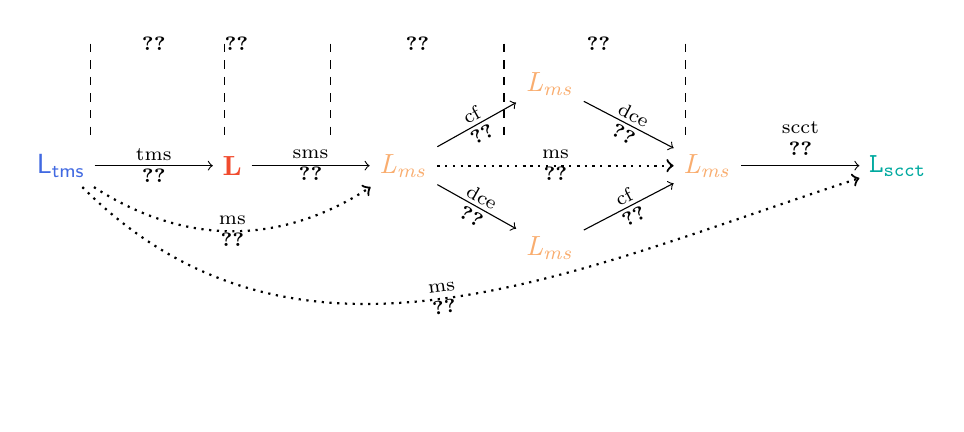
\begin{tikzpicture}
      \node (S) {$\src{L_{\tmssafe}}$};
      \node[right=1.5 of S] (T) {$\trg{L}$};
      \node[right=1.5 of T] (M) {$\irl{L_{\mssafe}}$};
      \node[below right=0.5 and 1.0 of M] (D0) {$\irl{L_{\mssafe}}$};
      \node[above right=0.5 and 1.0 of M] (C0) {$\irl{L_{\mssafe}}$};
      \node[right=3.0 of M] (E) {$\irl{L_{\mssafe}}$};
      \node[right=1.5 of E] (O) {$\obj{L_{\scctsafe}}$};

      \draw[->] (S) to[sloped] node[align=center,font=\scriptsize] (tmsedge) {\gls{tms}\\ \Cref{thm:cca:rtp:tms}} (T);
      \draw[->] (T) to[sloped] node[align=center,font=\scriptsize] {\gls{sms}\\ \Cref{thm:ccb:rtp:sms}} (M);
      \draw[->] (M) to[sloped] node[align=center,font=\scriptsize] {\gls{dce}\\ \Cref{thm:ccdce:rtp:ms}} (D0);
      \draw[->] (M) to[sloped] node[align=center,font=\scriptsize] {\gls{cf}\\ \Cref{thm:cccf:rtp:ms}} (C0);
      \draw[->] (D0) to[sloped] node[align=center,font=\scriptsize] {\gls{cf}\\ \Cref{thm:cccf:rtp:ms}} (E);
      \draw[->] (C0) to[sloped] node[align=center,font=\scriptsize] {\gls{dce}\\ \Cref{thm:ccdce:rtp:ms}} (E);
      \draw[->] (E) to[sloped,above] node[align=center,font=\scriptsize] {\gls{scct}\\ \Cref{thm:ccscct:rtp:scct}} (O);

      % Sections
      \node[above=1.0 of tmsedge] (sectms) {{\scriptsize\Cref{subsec:cs:tms}}};
      \node[right=0.5 of sectms] (secsms) {{\scriptsize\Cref{subsec:cs:ms}}};
      \node[right=1.75 of secsms] (secopts) {{\scriptsize\Cref{subsec:cs:opts}}};
      \node[right=1.75 of secopts] (secscct) {{\scriptsize\Cref{subsec:cs:scct}}};

      \draw[thick,dotted,->] (S) to[bend right=33,sloped] node[align=center,font=\scriptsize] {\gls{ms}\\ \Cref{thm:ccab:rtp:ms}} (M);
      \draw[thick,dotted,->] (M) to[bend right=0,sloped] node[align=center,font=\scriptsize] {\gls{ms}\\ \Cref{thm:cccfccdce:rtp:ms}} (E);
      \draw[thick,dotted,->] (S) to[out=-45,in=198,sloped] node[align=center,font=\scriptsize] {\gls{ms}\\ \Cref{thm:ccall:rtp:msscct}} (O);

      \draw[dashed] ($(sectms)-(0.8,0)$) -- ($(sectms)-(0.8,1.25)$);
      \draw[dashed] ($(sectms)-(-0.9,0)$) -- ($(sectms)-(-0.9,1.25)$);
      \draw[dashed] ($(secsms)-(-1.2,0)$) -- ($(secsms)-(-1.2,1.25)$);
      \draw[dashed] ($(secscct)-(1.2,0)$) -- ($(secscct)-(1.2,1.25)$);
      \draw[dashed] ($(secscct)-(-1.1,0)$) -- ($(secscct)-(-1.1,1.25)$);
    \end{tikzpicture}
  \end{center}
  \caption{Visualisation of the optimizing compilation pipeline that attains a combination of \gls{ms} and \gls{cct}.}\label{fig:pipeline}
\end{figure}
This section defines several secure compilers, each of which robustly preserves a different property of interest (\Cref{fig:pipeline}).
The power of the framework (\Cref{sec:compprop,sec:compcomp}) is demonstrated by composing these compilers for a secure, but optimizing, compilation chain that robustly preserves \gls{ms} and \gls{cct}.
Concretely, the section starts with a base-line definition for the used languages (\Cref{subsec:cs:defs}) and extends that to define languages $\src{L_{TMS}}$ and $\trg{L}$.
For programmers using $\src{L_{TMS}}$, their mental model should be that their code is temporal memory safe and cryptographic constant time.
The former is proven to be enforced by the static semantics of $\src{L_{TMS}}$, where each well-typed program is temporal memory safe.
The latter is completely untyped.
Having languages defined, this section continues with a compiler $\cc{\src{L_{\tmssafe}}}{\trg{L}}$ and proves that $\cc{\src{L_{\tmssafe}}}{\trg{L}}$ robustly preserves \gls{tms} (\Cref{subsec:cs:tms}).
For readability purposes, it defines $\irl{L_{MS}}$ to be exactly the same as $\trg{L}$ and continues to present a compiler $\cc{\trg{L}}{\irl{L_{MS}}}$ that robustly preserves \gls{sms} (\Cref{subsec:cs:ms}).
Now leaveraging the power of the framework that this paper introduces (\Cref{sec:compcomp,sec:compprop}), a compiler $\rtp{\cc{\src{L_{TMS}}}{\irl{L_{MS}}}}{\mssafe}$ is attained.
The next steps in the compilation pipeline are two secure compilers $\cc[_{\gls{dce}}]{\irl{L_{MS}}}{\irl{L_{MS}}}$ and $\cc[_{\gls{cf}}]{\irl{L_{MS}}}{\irl{L_{MS}}}$ that perform \glsfirst{dce} and \glsfirst{cf}, respectively, to model an optimzing pipeline happening somewhere in the compilation chain (\Cref{subsec:cs:opts}).
Finally, this section defines the language $\obj{L_{\scctsafe}}$ that is, in contrast to the other languages, not cryptographic constant time by definition.
Concluding, a compiler $\cc{\irl{L_{MS}}}{\obj{L_{CCT}}}$ that robustly preserves \gls{cct} (\Cref{subsec:cs:scct}) is shown and composed with $\cc{\src{L_{TMS}}}{\irl{L_{MS}}}$ and the optimizing compilers $\cc[_{\gls{dce}}]{\irl{L_{MS}}}{\irl{L_{MS}}}$ and $\cc[_{\gls{cf}}]{\irl{L_{MS}}}{\irl{L_{MS}}}$.
In turn, this yields $\cc{\src{L_{TMS}}}{\obj{L_{CCT}}}$, a compiler that robustly preserves a combination of \gls{ms} and \gls{cct}.



\subsection{Robust Temporal Memory Safety Preservation}\label{subsec:cs:tms}

\begin{center}
  $$
  \begin{array}{rcl}
%    \cca(\src{\lbinop{\expr[_{1}]}{\expr[_{2}]}}) & = & \lbinop[\trg]{\left[\cca(\src{\expr[_{1}]})\right]}{\left[\cca(\src{\expr[_{2}]})\right]} \\ [0.33cm]
    \cca(\src{\lfunction{g}{x:\natt\to\type[_{e}]}{\expr}}) & = & \lfunction[\trg]{\trg{g}}{\trg{x}}{\lifz[\trg]{\trg{\lhast{x}{\natt}}}{%
                                                                                                \left[\cca(\src{\expr})\right] %
                                                                                                 }{\labort[\trg]}}
  \end{array}
  $$
\end{center}

The only case where the compiler does something interesting is for top-level functions.
Here, a dynamic typecheck is inserted to respect the calling-convention.
Since $\trg{L}$ has no static typechecks, it could happen that a bogus context $\trg{\library_{\ctx}}$ calls a symbol accepting a $\src{\natt}$ with $\trg{\lpair{17}{29}}$.
The compiler ensures that execution does not proceed in cases like that.
This paper considers symbols on $\src{\natt}$.

\begin{theorem}[Compiler $\cca$ is secure with respect to \gls{tms}]\label{thm:cca:rtp:tms}
  $\rtp{\cca}{\tmssafe}$ % \Coqed
\end{theorem}

\begin{figure}[h]
  \begin{center}
    \begin{tikzpicture}[state/.style={minimum height=0.6cm}]
      % relative horizontal/vertical distance between states
      \pgfmathsetmacro{\hdist}{0.95}
      \pgfmathsetmacro{\vdist}{1.35}
      \pgfmathsetmacro{\halfvdist}{0.725}

      % row of src states
      \node[state] (srcempty) {$\src{\emptyset}$};
      \foreach \s [remember=\s as \cur (initially empty)] in {1,w_1,p,w_2,2} {
        \node[state,right=\hdist of src\cur] (src\s) {$\src{\Omega_{\s}}$};
      }
      % row of trg states
      \node[state,below=\vdist of srcempty] (trgempty) {$\trg{\emptyset}$};
      \foreach \s in {1,w_1,p,w_2,2} {
        \node[state,below=\vdist of src\s] (trg\s) {$\trg{\Omega_{\s}}$};
      }
      %% illustrations
        % backtrans wrapper 1
        \draw[thick,loosely dotted,Peach!50,rounded corners] (src1.north east) -- (srcw\string_1.north east)
          -- (trgw\string_1.south east) -- (trg1.south west) -- (src1.north west) -- cycle;
        % backtrans wrapper 2
        \draw[thick,loosely dotted,Peach!50,rounded corners] (srcp.north east) -- (srcw\string_2.north east)
          -- (trgw\string_2.south east) -- (trgp.south west) -- (srcp.north west) -- cycle;
        % compiler correctness
        \draw[thick,loosely dashed,Emerald!50,rounded corners] ($(srcw\string_1.north east)+(0,0.05)$) -- ($(srcp.north east)+(0,0.05)$)
          -- ($(trgw\string_2.north east)+(0.05,0)$) -- ($(trgw\string_2.south east)+(0.05,-0.05)$)
          -- ($(trg1.south west)+(-0.05,-0.05)$) -- ($(trg1.north west)+(-0.05,0)$) -- ($(srcw\string_1.north west)+(0,0.05)$) -- cycle;
      % state relations
      \path (srcempty) edge[draw=gray!25] node[pos=0.5,sloped,rotate=180,fill=white] {\scriptsize$\multimap_\emptyset$} (trgempty)
        (src1) edge[draw=gray!25] node[pos=0.5,sloped,rotate=180,fill=white] {\scriptsize$\multimap_{\delta_1}$} (trg1)
        (srcp) edge[draw=gray!25] node[pos=0.5,sloped,fill=white] {\scriptsize$\approx_{\delta_p}$} (trgp)
        (src2) edge[draw=gray!25] node[pos=0.5,sloped,rotate=180,fill=white] {\scriptsize$\multimap_{\delta_2}$} (trg2)
        (srcw\string_1) edge[draw=gray!25] node[pos=0.5,sloped,fill=white] {\scriptsize$\approx_{\delta_{w_1}}$} (trgw\string_1)
        (srcw\string_2) edge[draw=gray!25] node[pos=0.5,sloped,rotate=180,fill=white] {\scriptsize$\multimap_{\delta_{w_2}}$} (trgw\string_2)
        % diagonals
        (srcw\string_1) edge[draw=gray!25] node[pos=0.16,sloped,rotate=180,fill=white] {\scriptsize$\approx_{\delta_{w_1}}$} (trg1)
        (src1) edge[draw=gray!25] node[pos=0.16,sloped,rotate=180,fill=white] {\scriptsize$\multimap_{\delta_1}$} (trgw\string_1)
        (srcp) edge[draw=gray!25] node[pos=0.2,sloped,fill=white] {\scriptsize$\approx_{\delta_p}$} (trgw\string_2)
        (trgp) edge[draw=gray!25] node[pos=0.2,sloped,fill=white] {\scriptsize$\multimap_{\delta_{w_2}}$} (srcw\string_2)
        ;
      %\drawpolygon src1,srcw\string_1,trgw\string_1,trg1;
      %\drawpolygon srcp,srcw\string_2,trgw\string_2,trgp;
      %\node[font=\tiny,align=center,above=0.2 of srcw1srcp] (wrapper) {Backtranslation\\Wrapper};
      %\path[->,draw] (wrapper) -- (srcw\string_1);
      %\path[->,draw] (wrapper) -- (srcp);
      % steps
      \path[color=\stlccol] (srcempty) edge[draw=none] node {\ $\xrightarrow{\trace[_1]}{}{\kern-3.5pt}_{\text{ctx}}^*$} (src1)
        (src1) edge[draw=none] node {\ $\xrightarrow{\trace[_c]}{}{\kern-3.5pt}_{\text{ctx}}$} (srcw\string_1)
        (srcw\string_1) edge[draw=none] node {\ $\xrightarrow{\trace[_p]}{}{\kern-3.5pt}_{\text{ctx}}^*$} (srcp)
        (srcp) edge[draw=none] node[fill=white,inner sep=0,outer sep=0] {\ $\xrightarrow{\trace[_r]}{}{\kern-3.5pt}_{\text{ctx}}$} (srcw\string_2)
        (srcw\string_2) edge[draw=none] node {\ $\xrightarrow{\trace[_2]}{}{\kern-3.5pt}_{\text{ctx}}^*$} (src2)
        ;
      \path[color=\ulccol] (trgempty) edge[draw=none] node[fill=white,inner sep=0,outer sep=0] {\ $\xrightarrow{\phantom{\trace[_1]}}{}{\kern-3.5pt}_{\text{ctx}}^*$} (trg1)
        (trg1) edge[draw=none] node {\ $\xrightarrow{\phantom{\trace[_p]}}{}{\kern-3.5pt}_{\text{ctx}}^*$} (trgw\string_1)
        (trgw\string_1) edge[draw=none] node[fill=white,inner sep=0,outer sep=0] {\ $\xrightarrow{\phantom{\trace[_p]}}{}{\kern-3.5pt}_{\text{ctx}}^*$} (trgp)
        (trgp) edge[draw=none] node {\ $\xrightarrow{\phantom{\trace[_p]}}{}{\kern-3.5pt}_{\text{ctx}}^*$} (trgw\string_2)
        (trgw\string_2) edge[draw=none] node {\ $\xrightarrow{\phantom{\trace[_2]}}{}{\kern-3.5pt}_{\text{ctx}}^*$} (trg2)
        ;
      % legend
      \node[align=left,below right=0.3 and 0.3 of trgempty,font=\tiny] (legend) {%
        ${\src{\trace[_c]}}\cong{\backt{\Ltms}{\Ltrg}(\trg{Call\ ?\finalexpr_i})}$\\%
        ${\src{\trace[_r]}}\cong{\backt{\Ltms}{\Ltrg}(\trg{Ret\ !\finalexpr_o})}$
        };
      \draw[thick,loosely dotted,Peach!50,rounded corners] ($(legend.north east)+(0.5,-0.4)$) -- ($(legend.north east)+(1,-0.4)$);
      \node at ($(legend.north east)+(1.5,-0.4)$) (legendwrapper) {};
      \node[right of=legendwrapper] {\tiny Backtranslation Wrapper};
      \draw[thick,loosely dashed,Emerald!50,rounded corners] ($(legend.south east)+(0.5,0.4)$) -- ($(legend.south east)+(1,0.4)$);
      \node at ($(legend.south east)+(1.5,0.4)$) (legendcorrectness) {};
      \node[right of=legendcorrectness] {\tiny Compiler Correctness};
    \end{tikzpicture}
    \caption{Proof diagram for \Cref{thm:cca:rtp:tms} depicting the general structure of robust preservation proofs.}\label{fig:proofdiag:rtp}
  \end{center}
\end{figure}

\subsection{Robust (Spatial) Memory Safety Preservation}\label{subsec:cs:ms}

In this section, the language $\irl{L_{\mssafe}}$ is exactly the same as $\trg{L}$ and are considered equal.
However, it is still named and collored differently to emphasize the fact that after this section, compiled $\irl{L_{\mssafe}}$ programs are \gls{ms}.

\begin{center}
  $$
  \begin{array}{rcl}
    \ccb(\trg{\lnew{x}{\expr[_{1}]}{\expr[_{2}]}}) & = & \llet[\irl]{\irl{x_{SIZE}}}{\ccb(\trg{\expr[_{1}]})}{\lnew[\irl]{\irl{x}}{\irl{x_{SIZE}}}{\ccb(\trg{\expr[_{2}]})}} \\
    \ccb(\trg{\lget{x}{\expr}}) & = & \llet[\irl]{\irl{x_{n}}}{\ccb(\trg{\expr})}{\irl{\lifz{0\le x_{n}<x_{SIZE}}{\lget{x}{x_{n}}}{\labort}}} \\
    \ccb(\trg{\lset{x}{\expr[_{1}]}{\expr[_{2}]}}) & = & \llet[\irl]{\irl{x_{n}}}{\ccb(\trg{\expr[_{1}]})}{\lifz[\irl]{\irl{0\le x_{n}<x_{SIZE}}}{\lset[\irl]{\irl{x}}{\irl{x_{n}}}{\ccb(\trg{\expr[_{2}]})}}{\irl{\labort}}} \\
  \end{array}
  $$
\end{center}

Up to getting and setting memory, the compiler is the identity function.
For memory accesses, however, a bounds--check is inserted that enforces \gls{sms}.
To this end, the compiler introduces another, fresh identifier $\irl{x_{SIZE}}$ for each allocation that binds $\irl{x}$ to keep track of the allocation size.

\begin{theorem}[Compiler $\ccb$ is secure with respect to \gls{sms}]\label{thm:ccb:rtp:sms}
  $\rtp{\ccb}{\smssafe}$ % \Coqed
\end{theorem}

The composition of $\cca$ and $\ccb$ attains full memory safety using \Cref{thm:rtp,thm:cca:rtp:tms,thm:ccb:rtp:sms}.

\begin{theorem}[Compiler $\cca\circ\ccb$ is secure with respect to \gls{ms}]\label{thm:ccab:rtp:ms}
  $\rtp{\cca\circ\ccb}{\mssafe}$ % \Coqed
\end{theorem}

\subsection{Optimizing Compilers}\label{subsec:cs:opts}

\begin{center}
  $$
  \begin{array}{rcl}
    \ccdce(\irl{\lifz{true}{\expr[_{1}]}{\expr[_{2}]}}) & = & \ccdce(\irl{\expr[_{1}]}) \\
    \ccdce(\irl{\lifz{false}{\expr[_{1}]}{\expr[_{2}]}}) & = & \ccdce(\irl{\expr[_{2}]}) \\
  \end{array}
  $$
\end{center}

\begin{center}
  $$
  \begin{array}{rcll}
    \cccf(\irl{\llet{x}{n}{\expr}}) & = & \cccf(\irl{\expr\subst{n}{x}}) &\\
    \cccf(\irl{\lbinop{n_{1}}{n_{2}}}) & = & \irl{n_{3}} & \text{where }\irl{n_{3}}\text{ is }\lbinop{\irl{n_{1}}}{\irl{n_{2}}}\\
  \end{array}
  $$
\end{center}

\begin{theorem}[Compiler $\ccdce$ is secure with respect to \gls{ms}]\label{thm:ccdce:rtp:ms}
  $\rtp{\ccdce}{\mssafe}$ % \Coqed
\end{theorem}
\begin{theorem}[Compiler $\cccf$ is secure with respect to \gls{ms}]\label{thm:cccf:rtp:ms}
  $\rtp{\cccf}{\mssafe}$ % \Coqed
\end{theorem}

\begin{theorem}[Compilers $\cccf\circ\ccdce$ and $\cccf\circ\ccdce$ are secure with respect to \gls{ms}]\label{thm:cccfccdce:rtp:ms}
  $\rtp{\cccf\circ\ccdce}{\mssafe}$ and $\rtp{\ccdce\circ\cccf}{\mssafe}$ % \Coqed
\end{theorem}

\subsection{Robust Strict Cryptographic Constant Time Preservation}\label{subsec:cs:scct}

\begin{center}
  $$
  \begin{array}{rcl}
    \ccscct(\irl{\lfunction{g}{x}{\expr}}) & = & \lfunction[\obj]{\obj{g}}{\obj{x}}{\obj{\lwrdoit{1};}\ccscct(\irl{\expr})}
  \end{array}
  $$
\end{center}

\begin{theorem}[Compiler $\ccscct$ is secure with respect to \gls{scct}]\label{thm:ccscct:rtp:scct}
  $\rtp{\ccscct}{\scctsafe}$ % \Coqed
\end{theorem}

\subsection{Robust Preservation of Intersection of Memory Safety and Strict Cryptographic Constant Time}

Let $\cc{\Ltms}{\Lscct}$ be the compiler that is the composition of $\cca$, $\ccb$, $\cccf$, $\ccdce$, and $\ccscct$, then the following theorem can be shown.

\begin{theorem}[Compiler $\ccscct$ is secure with respect to \gls{scct}]\label{thm:ccscct:rtp:scct}
  $\rtp{\ccscct}{\scctsafe}$ % \Coqed
\end{theorem}

\begin{theorem}[Compiler $\ccscct$ is secure with respect to \gls{scct}]\label{thm:ccall:rtp:msscct}
  $\rtp{\cc{\Ltms}{\Lscct}}{\mssafe\cap\scctsafe}$ % \Coqed
\end{theorem}

%\begin{lstlisting}[language=c,caption=``Wrong bounds check of two 64-bit integers.'']
%if at <= bounds {
%  x[at] = 42;
%}
%\end{lstlisting}
%Note the subtle bug of using \verb|<=| instead of \verb|<|, leading to an out-of-bounds access whenever \verb|at = bounds|.
%Furthermore, when \verb|at| and \verb|bounds| are 64-bit integers on a 32-bit architecture, the comparison may not be performed in constant-time: The compiler may bail out as soon as the lower 32 bits are unequal, not bothering to compare the higher 32 bits.


\section{Related Work}\label{sec:relwork}

This section compares existing work with the one presented in this paper.
To this end, work on robust preservation criteria (\Cref{subsec:relw:seccomprtp}) and on other secure compiler criteria (\Cref{subsec:relw:seccompcrit}) is being looked at.
The case study of this paper (\Cref{sec:casestud:defs,sec:casestud:rtp}) implements measures for ensuring \gls{ms} as well as \gls{cct} and these are compared with previous work as well (\Cref{subsec:relw:msmechs,subsec:relw:cctmechs}).

\subsection{Secure Compilation as Robust Preservation}\label{subsec:relw:seccomprtp}

The robust preservation of properties as a compiler--level criterion has been analyzed extensively~\cite{abate2019jour,patrignani2021rsc,abate2021extacc,patrignani2022universal,patrignani2019survey,kruse2022csc}.
This work has made use of that previous work and formalized the compositionality aspect which has not been explored before.
While there exists a composition theorem~\cite{abate2019jour} already, that theorem is not concerned with composing robustly safe compilers, but rather program components and contexts.
The work relating robust preservation with universal composability~\cite{patrignani2022universal} is closest to what this paper presents.
The authors demonstrate a similar compositionality theorem to what is presented here (\Cref{sec:compcomp}).
However, they do not demonstrate the scalability of the approach in the context of a practical compilation chain.

\subsection{Other Secure Compilation Criteria}\label{subsec:relw:seccompcrit}

\MKin{category theory stuff}
\MKin{full abstraction -> not compositional}
\MKin{compositional compiler correctness?}

\subsection{Memory Safety Mechanisms}\label{subsec:relw:msmechs}

\cite{michael2023mswasm}

\subsection{Cryptographic Constant Time Mechanisms}\label{subsec:relw:cctmechs}

\section{Conclusion}\label{sec:concl}


%% The acknowledgments section is defined using the "acks" environment
%% (and NOT an unnumbered section). This ensures the proper
%% identification of the section in the article metadata, and the
%% consistent spelling of the heading.
\begin{acks}
\end{acks}

%%
%% The next two lines define the bibliography style to be used, and
%% the bibliography file.
\bibliographystyle{ACM-Reference-Format}
\bibliography{main}

%%
%% If your work has an appendix, this is the place to put it.
\appendix

\end{document}
\endinput
%%
%% End of file `sample-sigconf.tex'.
